\documentclass{article}
\usepackage[final]{neurips_2025}  % NEURIPS style (neurips_2025.sty is in paper_draft/)
% neurips_2025.sty with [final] alone leaves \@trackname undefined (it is set only by a track option).
% Define the footer notice here; swap in a track option (e.g. [main, final]) for a real submission.
\makeatletter\providecommand{\@trackname}{Preprint. Not peer reviewed.}\makeatother
\usepackage[hidelinks]{hyperref}  % REQUIRED: clickable links
\usepackage{booktabs}  % REQUIRED: professional tables
\usepackage{graphicx}
\usepackage{amsmath,amssymb}
\usepackage[utf8]{inputenc}
\usepackage[T1]{fontenc}
\usepackage{enumitem}
\usepackage{multirow}
\usepackage{algorithm}
\usepackage[noend]{algpseudocode}

% Import command files
%%%%% MATH NOTATION MACROS %%%%%
% Standard math notation for academic papers
% Import with: %%%%% MATH NOTATION MACROS %%%%%
% Standard math notation for academic papers
% Import with: %%%%% MATH NOTATION MACROS %%%%%
% Standard math notation for academic papers
% Import with: \input{commands/math}

\usepackage{amsmath,amsfonts,bm}

%%%%%%%%%%%%%%%%%%%%%%%%%%%%%%%%%%%%%%%%%%%%%%%%%%%%%%%%%%%%%%%%%
% FIGURE AND SECTION REFERENCES
%%%%%%%%%%%%%%%%%%%%%%%%%%%%%%%%%%%%%%%%%%%%%%%%%%%%%%%%%%%%%%%%%

% Mark sections of captions for referring to divisions of figures
\newcommand{\figleft}{{\em (Left)}}
\newcommand{\figcenter}{{\em (Center)}}
\newcommand{\figright}{{\em (Right)}}
\newcommand{\figtop}{{\em (Top)}}
\newcommand{\figbottom}{{\em (Bottom)}}
\newcommand{\captiona}{{\em (a)}}
\newcommand{\captionb}{{\em (b)}}
\newcommand{\captionc}{{\em (c)}}
\newcommand{\captiond}{{\em (d)}}

% Figure references
\def\figref#1{figure~\ref{#1}}
\def\Figref#1{Figure~\ref{#1}}
\def\twofigref#1#2{figures \ref{#1} and \ref{#2}}
\def\quadfigref#1#2#3#4{figures \ref{#1}, \ref{#2}, \ref{#3} and \ref{#4}}

% Section references
\def\secref#1{section~\ref{#1}}
\def\Secref#1{Section~\ref{#1}}
\def\twosecrefs#1#2{sections \ref{#1} and \ref{#2}}
\def\secrefs#1#2#3{sections \ref{#1}, \ref{#2} and \ref{#3}}

% Equation references
\def\eqref#1{equation~\ref{#1}}
\def\Eqref#1{Equation~\ref{#1}}
\def\plaineqref#1{\ref{#1}}

% Algorithm references
\def\algref#1{algorithm~\ref{#1}}
\def\Algref#1{Algorithm~\ref{#1}}
\def\twoalgref#1#2{algorithms \ref{#1} and \ref{#2}}
\def\Twoalgref#1#2{Algorithms \ref{#1} and \ref{#2}}

% Table references
\def\tabref#1{table~\ref{#1}}
\def\Tabref#1{Table~\ref{#1}}

% Chapter references
\def\chapref#1{chapter~\ref{#1}}
\def\Chapref#1{Chapter~\ref{#1}}

%%%%%%%%%%%%%%%%%%%%%%%%%%%%%%%%%%%%%%%%%%%%%%%%%%%%%%%%%%%%%%%%%
% BASIC MATH DEFINITIONS
%%%%%%%%%%%%%%%%%%%%%%%%%%%%%%%%%%%%%%%%%%%%%%%%%%%%%%%%%%%%%%%%%

\def\ceil#1{\lceil #1 \rceil}
\def\floor#1{\lfloor #1 \rfloor}
\def\1{\bm{1}}
\def\eps{{\epsilon}}

% Common operators
\DeclareMathOperator*{\argmax}{arg\,max}
\DeclareMathOperator*{\argmin}{arg\,min}
\DeclareMathOperator{\sign}{sign}
\DeclareMathOperator{\Tr}{Tr}
\let\ab\allowbreak

%%%%%%%%%%%%%%%%%%%%%%%%%%%%%%%%%%%%%%%%%%%%%%%%%%%%%%%%%%%%%%%%%
% VECTORS (lowercase bold)
%%%%%%%%%%%%%%%%%%%%%%%%%%%%%%%%%%%%%%%%%%%%%%%%%%%%%%%%%%%%%%%%%

\def\vzero{{\bm{0}}}
\def\vone{{\bm{1}}}
\def\vmu{{\bm{\mu}}}
\def\vtheta{{\bm{\theta}}}
\def\va{{\bm{a}}}
\def\vb{{\bm{b}}}
\def\vc{{\bm{c}}}
\def\vd{{\bm{d}}}
\def\ve{{\bm{e}}}
\def\vf{{\bm{f}}}
\def\vg{{\bm{g}}}
\def\vh{{\bm{h}}}
\def\vi{{\bm{i}}}
\def\vj{{\bm{j}}}
\def\vk{{\bm{k}}}
\def\vl{{\bm{l}}}
\def\vm{{\bm{m}}}
\def\vn{{\bm{n}}}
\def\vo{{\bm{o}}}
\def\vp{{\bm{p}}}
\def\vq{{\bm{q}}}
\def\vr{{\bm{r}}}
\def\vs{{\bm{s}}}
\def\vt{{\bm{t}}}
\def\vu{{\bm{u}}}
\def\vv{{\bm{v}}}
\def\vw{{\bm{w}}}
\def\vx{{\bm{x}}}
\def\vy{{\bm{y}}}
\def\vz{{\bm{z}}}

%%%%%%%%%%%%%%%%%%%%%%%%%%%%%%%%%%%%%%%%%%%%%%%%%%%%%%%%%%%%%%%%%
% MATRICES (uppercase bold)
%%%%%%%%%%%%%%%%%%%%%%%%%%%%%%%%%%%%%%%%%%%%%%%%%%%%%%%%%%%%%%%%%

\def\mA{{\bm{A}}}
\def\mB{{\bm{B}}}
\def\mC{{\bm{C}}}
\def\mD{{\bm{D}}}
\def\mE{{\bm{E}}}
\def\mF{{\bm{F}}}
\def\mG{{\bm{G}}}
\def\mH{{\bm{H}}}
\def\mI{{\bm{I}}}
\def\mJ{{\bm{J}}}
\def\mK{{\bm{K}}}
\def\mL{{\bm{L}}}
\def\mM{{\bm{M}}}
\def\mN{{\bm{N}}}
\def\mO{{\bm{O}}}
\def\mP{{\bm{P}}}
\def\mQ{{\bm{Q}}}
\def\mR{{\bm{R}}}
\def\mS{{\bm{S}}}
\def\mT{{\bm{T}}}
\def\mU{{\bm{U}}}
\def\mV{{\bm{V}}}
\def\mW{{\bm{W}}}
\def\mX{{\bm{X}}}
\def\mY{{\bm{Y}}}
\def\mZ{{\bm{Z}}}
\def\mBeta{{\bm{\beta}}}
\def\mPhi{{\bm{\Phi}}}
\def\mLambda{{\bm{\Lambda}}}
\def\mSigma{{\bm{\Sigma}}}

%%%%%%%%%%%%%%%%%%%%%%%%%%%%%%%%%%%%%%%%%%%%%%%%%%%%%%%%%%%%%%%%%
% CALLIGRAPHIC (mathcal)
%%%%%%%%%%%%%%%%%%%%%%%%%%%%%%%%%%%%%%%%%%%%%%%%%%%%%%%%%%%%%%%%%

\def\gA{{\mathcal{A}}}
\def\gB{{\mathcal{B}}}
\def\gC{{\mathcal{C}}}
\def\gD{{\mathcal{D}}}
\def\gE{{\mathcal{E}}}
\def\gF{{\mathcal{F}}}
\def\gG{{\mathcal{G}}}
\def\gH{{\mathcal{H}}}
\def\gI{{\mathcal{I}}}
\def\gJ{{\mathcal{J}}}
\def\gK{{\mathcal{K}}}
\def\gL{{\mathcal{L}}}
\def\gM{{\mathcal{M}}}
\def\gN{{\mathcal{N}}}
\def\gO{{\mathcal{O}}}
\def\gP{{\mathcal{P}}}
\def\gQ{{\mathcal{Q}}}
\def\gR{{\mathcal{R}}}
\def\gS{{\mathcal{S}}}
\def\gT{{\mathcal{T}}}
\def\gU{{\mathcal{U}}}
\def\gV{{\mathcal{V}}}
\def\gW{{\mathcal{W}}}
\def\gX{{\mathcal{X}}}
\def\gY{{\mathcal{Y}}}
\def\gZ{{\mathcal{Z}}}

%%%%%%%%%%%%%%%%%%%%%%%%%%%%%%%%%%%%%%%%%%%%%%%%%%%%%%%%%%%%%%%%%
% SETS (blackboard bold)
%%%%%%%%%%%%%%%%%%%%%%%%%%%%%%%%%%%%%%%%%%%%%%%%%%%%%%%%%%%%%%%%%

\def\sA{{\mathbb{A}}}
\def\sB{{\mathbb{B}}}
\def\sC{{\mathbb{C}}}
\def\sD{{\mathbb{D}}}
\def\sF{{\mathbb{F}}}
\def\sG{{\mathbb{G}}}
\def\sH{{\mathbb{H}}}
\def\sI{{\mathbb{I}}}
\def\sJ{{\mathbb{J}}}
\def\sK{{\mathbb{K}}}
\def\sL{{\mathbb{L}}}
\def\sM{{\mathbb{M}}}
\def\sN{{\mathbb{N}}}
\def\sO{{\mathbb{O}}}
\def\sP{{\mathbb{P}}}
\def\sQ{{\mathbb{Q}}}
\def\sR{{\mathbb{R}}}
\def\sS{{\mathbb{S}}}
\def\sT{{\mathbb{T}}}
\def\sU{{\mathbb{U}}}
\def\sV{{\mathbb{V}}}
\def\sW{{\mathbb{W}}}
\def\sX{{\mathbb{X}}}
\def\sY{{\mathbb{Y}}}
\def\sZ{{\mathbb{Z}}}

%%%%%%%%%%%%%%%%%%%%%%%%%%%%%%%%%%%%%%%%%%%%%%%%%%%%%%%%%%%%%%%%%
% COMMON MATH SHORTCUTS
%%%%%%%%%%%%%%%%%%%%%%%%%%%%%%%%%%%%%%%%%%%%%%%%%%%%%%%%%%%%%%%%%

% Expectation and variance
\newcommand{\E}{\mathbb{E}}
\newcommand{\Var}{\mathrm{Var}}
\newcommand{\Cov}{\mathrm{Cov}}
\newcommand{\R}{\mathbb{R}}

% Datasets
\newcommand{\train}{\mathcal{D}}
\newcommand{\valid}{\mathcal{D_{\mathrm{valid}}}}
\newcommand{\test}{\mathcal{D_{\mathrm{test}}}}

% Distributions
\newcommand{\laplace}{\mathrm{Laplace}}
\newcommand{\Uniform}{\mathrm{Unif}}
\newcommand{\Normal}{\mathrm{Normal}}
\newcommand{\Categorical}{\mathrm{Categorical}}

% Common functions
\newcommand{\softmax}{\mathrm{softmax}}
\newcommand{\sigmoid}{\sigma}
\newcommand{\KL}{D_{\mathrm{KL}}}

% Norms
\newcommand{\normlzero}{L^0}
\newcommand{\normlone}{L^1}
\newcommand{\normltwo}{L^2}
\newcommand{\normlp}{L^p}
\newcommand{\normmax}{L^\infty}

%%%%%%%%%%%%%%%%%%%%%%%%%%%%%%%%%%%%%%%%%%%%%%%%%%%%%%%%%%%%%%%%%
% DEFINITIONS AND HIGHLIGHTING
%%%%%%%%%%%%%%%%%%%%%%%%%%%%%%%%%%%%%%%%%%%%%%%%%%%%%%%%%%%%%%%%%

% Highlight a newly defined term
\newcommand{\newterm}[1]{{\bf #1}}
\newcommand{\defn}[1]{\textbf{#1}}
\newcommand{\defeq}{\mathrel{\stackrel{\textnormal{\tiny def}}{=}}}


\usepackage{amsmath,amsfonts,bm}

%%%%%%%%%%%%%%%%%%%%%%%%%%%%%%%%%%%%%%%%%%%%%%%%%%%%%%%%%%%%%%%%%
% FIGURE AND SECTION REFERENCES
%%%%%%%%%%%%%%%%%%%%%%%%%%%%%%%%%%%%%%%%%%%%%%%%%%%%%%%%%%%%%%%%%

% Mark sections of captions for referring to divisions of figures
\newcommand{\figleft}{{\em (Left)}}
\newcommand{\figcenter}{{\em (Center)}}
\newcommand{\figright}{{\em (Right)}}
\newcommand{\figtop}{{\em (Top)}}
\newcommand{\figbottom}{{\em (Bottom)}}
\newcommand{\captiona}{{\em (a)}}
\newcommand{\captionb}{{\em (b)}}
\newcommand{\captionc}{{\em (c)}}
\newcommand{\captiond}{{\em (d)}}

% Figure references
\def\figref#1{figure~\ref{#1}}
\def\Figref#1{Figure~\ref{#1}}
\def\twofigref#1#2{figures \ref{#1} and \ref{#2}}
\def\quadfigref#1#2#3#4{figures \ref{#1}, \ref{#2}, \ref{#3} and \ref{#4}}

% Section references
\def\secref#1{section~\ref{#1}}
\def\Secref#1{Section~\ref{#1}}
\def\twosecrefs#1#2{sections \ref{#1} and \ref{#2}}
\def\secrefs#1#2#3{sections \ref{#1}, \ref{#2} and \ref{#3}}

% Equation references
\def\eqref#1{equation~\ref{#1}}
\def\Eqref#1{Equation~\ref{#1}}
\def\plaineqref#1{\ref{#1}}

% Algorithm references
\def\algref#1{algorithm~\ref{#1}}
\def\Algref#1{Algorithm~\ref{#1}}
\def\twoalgref#1#2{algorithms \ref{#1} and \ref{#2}}
\def\Twoalgref#1#2{Algorithms \ref{#1} and \ref{#2}}

% Table references
\def\tabref#1{table~\ref{#1}}
\def\Tabref#1{Table~\ref{#1}}

% Chapter references
\def\chapref#1{chapter~\ref{#1}}
\def\Chapref#1{Chapter~\ref{#1}}

%%%%%%%%%%%%%%%%%%%%%%%%%%%%%%%%%%%%%%%%%%%%%%%%%%%%%%%%%%%%%%%%%
% BASIC MATH DEFINITIONS
%%%%%%%%%%%%%%%%%%%%%%%%%%%%%%%%%%%%%%%%%%%%%%%%%%%%%%%%%%%%%%%%%

\def\ceil#1{\lceil #1 \rceil}
\def\floor#1{\lfloor #1 \rfloor}
\def\1{\bm{1}}
\def\eps{{\epsilon}}

% Common operators
\DeclareMathOperator*{\argmax}{arg\,max}
\DeclareMathOperator*{\argmin}{arg\,min}
\DeclareMathOperator{\sign}{sign}
\DeclareMathOperator{\Tr}{Tr}
\let\ab\allowbreak

%%%%%%%%%%%%%%%%%%%%%%%%%%%%%%%%%%%%%%%%%%%%%%%%%%%%%%%%%%%%%%%%%
% VECTORS (lowercase bold)
%%%%%%%%%%%%%%%%%%%%%%%%%%%%%%%%%%%%%%%%%%%%%%%%%%%%%%%%%%%%%%%%%

\def\vzero{{\bm{0}}}
\def\vone{{\bm{1}}}
\def\vmu{{\bm{\mu}}}
\def\vtheta{{\bm{\theta}}}
\def\va{{\bm{a}}}
\def\vb{{\bm{b}}}
\def\vc{{\bm{c}}}
\def\vd{{\bm{d}}}
\def\ve{{\bm{e}}}
\def\vf{{\bm{f}}}
\def\vg{{\bm{g}}}
\def\vh{{\bm{h}}}
\def\vi{{\bm{i}}}
\def\vj{{\bm{j}}}
\def\vk{{\bm{k}}}
\def\vl{{\bm{l}}}
\def\vm{{\bm{m}}}
\def\vn{{\bm{n}}}
\def\vo{{\bm{o}}}
\def\vp{{\bm{p}}}
\def\vq{{\bm{q}}}
\def\vr{{\bm{r}}}
\def\vs{{\bm{s}}}
\def\vt{{\bm{t}}}
\def\vu{{\bm{u}}}
\def\vv{{\bm{v}}}
\def\vw{{\bm{w}}}
\def\vx{{\bm{x}}}
\def\vy{{\bm{y}}}
\def\vz{{\bm{z}}}

%%%%%%%%%%%%%%%%%%%%%%%%%%%%%%%%%%%%%%%%%%%%%%%%%%%%%%%%%%%%%%%%%
% MATRICES (uppercase bold)
%%%%%%%%%%%%%%%%%%%%%%%%%%%%%%%%%%%%%%%%%%%%%%%%%%%%%%%%%%%%%%%%%

\def\mA{{\bm{A}}}
\def\mB{{\bm{B}}}
\def\mC{{\bm{C}}}
\def\mD{{\bm{D}}}
\def\mE{{\bm{E}}}
\def\mF{{\bm{F}}}
\def\mG{{\bm{G}}}
\def\mH{{\bm{H}}}
\def\mI{{\bm{I}}}
\def\mJ{{\bm{J}}}
\def\mK{{\bm{K}}}
\def\mL{{\bm{L}}}
\def\mM{{\bm{M}}}
\def\mN{{\bm{N}}}
\def\mO{{\bm{O}}}
\def\mP{{\bm{P}}}
\def\mQ{{\bm{Q}}}
\def\mR{{\bm{R}}}
\def\mS{{\bm{S}}}
\def\mT{{\bm{T}}}
\def\mU{{\bm{U}}}
\def\mV{{\bm{V}}}
\def\mW{{\bm{W}}}
\def\mX{{\bm{X}}}
\def\mY{{\bm{Y}}}
\def\mZ{{\bm{Z}}}
\def\mBeta{{\bm{\beta}}}
\def\mPhi{{\bm{\Phi}}}
\def\mLambda{{\bm{\Lambda}}}
\def\mSigma{{\bm{\Sigma}}}

%%%%%%%%%%%%%%%%%%%%%%%%%%%%%%%%%%%%%%%%%%%%%%%%%%%%%%%%%%%%%%%%%
% CALLIGRAPHIC (mathcal)
%%%%%%%%%%%%%%%%%%%%%%%%%%%%%%%%%%%%%%%%%%%%%%%%%%%%%%%%%%%%%%%%%

\def\gA{{\mathcal{A}}}
\def\gB{{\mathcal{B}}}
\def\gC{{\mathcal{C}}}
\def\gD{{\mathcal{D}}}
\def\gE{{\mathcal{E}}}
\def\gF{{\mathcal{F}}}
\def\gG{{\mathcal{G}}}
\def\gH{{\mathcal{H}}}
\def\gI{{\mathcal{I}}}
\def\gJ{{\mathcal{J}}}
\def\gK{{\mathcal{K}}}
\def\gL{{\mathcal{L}}}
\def\gM{{\mathcal{M}}}
\def\gN{{\mathcal{N}}}
\def\gO{{\mathcal{O}}}
\def\gP{{\mathcal{P}}}
\def\gQ{{\mathcal{Q}}}
\def\gR{{\mathcal{R}}}
\def\gS{{\mathcal{S}}}
\def\gT{{\mathcal{T}}}
\def\gU{{\mathcal{U}}}
\def\gV{{\mathcal{V}}}
\def\gW{{\mathcal{W}}}
\def\gX{{\mathcal{X}}}
\def\gY{{\mathcal{Y}}}
\def\gZ{{\mathcal{Z}}}

%%%%%%%%%%%%%%%%%%%%%%%%%%%%%%%%%%%%%%%%%%%%%%%%%%%%%%%%%%%%%%%%%
% SETS (blackboard bold)
%%%%%%%%%%%%%%%%%%%%%%%%%%%%%%%%%%%%%%%%%%%%%%%%%%%%%%%%%%%%%%%%%

\def\sA{{\mathbb{A}}}
\def\sB{{\mathbb{B}}}
\def\sC{{\mathbb{C}}}
\def\sD{{\mathbb{D}}}
\def\sF{{\mathbb{F}}}
\def\sG{{\mathbb{G}}}
\def\sH{{\mathbb{H}}}
\def\sI{{\mathbb{I}}}
\def\sJ{{\mathbb{J}}}
\def\sK{{\mathbb{K}}}
\def\sL{{\mathbb{L}}}
\def\sM{{\mathbb{M}}}
\def\sN{{\mathbb{N}}}
\def\sO{{\mathbb{O}}}
\def\sP{{\mathbb{P}}}
\def\sQ{{\mathbb{Q}}}
\def\sR{{\mathbb{R}}}
\def\sS{{\mathbb{S}}}
\def\sT{{\mathbb{T}}}
\def\sU{{\mathbb{U}}}
\def\sV{{\mathbb{V}}}
\def\sW{{\mathbb{W}}}
\def\sX{{\mathbb{X}}}
\def\sY{{\mathbb{Y}}}
\def\sZ{{\mathbb{Z}}}

%%%%%%%%%%%%%%%%%%%%%%%%%%%%%%%%%%%%%%%%%%%%%%%%%%%%%%%%%%%%%%%%%
% COMMON MATH SHORTCUTS
%%%%%%%%%%%%%%%%%%%%%%%%%%%%%%%%%%%%%%%%%%%%%%%%%%%%%%%%%%%%%%%%%

% Expectation and variance
\newcommand{\E}{\mathbb{E}}
\newcommand{\Var}{\mathrm{Var}}
\newcommand{\Cov}{\mathrm{Cov}}
\newcommand{\R}{\mathbb{R}}

% Datasets
\newcommand{\train}{\mathcal{D}}
\newcommand{\valid}{\mathcal{D_{\mathrm{valid}}}}
\newcommand{\test}{\mathcal{D_{\mathrm{test}}}}

% Distributions
\newcommand{\laplace}{\mathrm{Laplace}}
\newcommand{\Uniform}{\mathrm{Unif}}
\newcommand{\Normal}{\mathrm{Normal}}
\newcommand{\Categorical}{\mathrm{Categorical}}

% Common functions
\newcommand{\softmax}{\mathrm{softmax}}
\newcommand{\sigmoid}{\sigma}
\newcommand{\KL}{D_{\mathrm{KL}}}

% Norms
\newcommand{\normlzero}{L^0}
\newcommand{\normlone}{L^1}
\newcommand{\normltwo}{L^2}
\newcommand{\normlp}{L^p}
\newcommand{\normmax}{L^\infty}

%%%%%%%%%%%%%%%%%%%%%%%%%%%%%%%%%%%%%%%%%%%%%%%%%%%%%%%%%%%%%%%%%
% DEFINITIONS AND HIGHLIGHTING
%%%%%%%%%%%%%%%%%%%%%%%%%%%%%%%%%%%%%%%%%%%%%%%%%%%%%%%%%%%%%%%%%

% Highlight a newly defined term
\newcommand{\newterm}[1]{{\bf #1}}
\newcommand{\defn}[1]{\textbf{#1}}
\newcommand{\defeq}{\mathrel{\stackrel{\textnormal{\tiny def}}{=}}}


\usepackage{amsmath,amsfonts,bm}

%%%%%%%%%%%%%%%%%%%%%%%%%%%%%%%%%%%%%%%%%%%%%%%%%%%%%%%%%%%%%%%%%
% FIGURE AND SECTION REFERENCES
%%%%%%%%%%%%%%%%%%%%%%%%%%%%%%%%%%%%%%%%%%%%%%%%%%%%%%%%%%%%%%%%%

% Mark sections of captions for referring to divisions of figures
\newcommand{\figleft}{{\em (Left)}}
\newcommand{\figcenter}{{\em (Center)}}
\newcommand{\figright}{{\em (Right)}}
\newcommand{\figtop}{{\em (Top)}}
\newcommand{\figbottom}{{\em (Bottom)}}
\newcommand{\captiona}{{\em (a)}}
\newcommand{\captionb}{{\em (b)}}
\newcommand{\captionc}{{\em (c)}}
\newcommand{\captiond}{{\em (d)}}

% Figure references
\def\figref#1{figure~\ref{#1}}
\def\Figref#1{Figure~\ref{#1}}
\def\twofigref#1#2{figures \ref{#1} and \ref{#2}}
\def\quadfigref#1#2#3#4{figures \ref{#1}, \ref{#2}, \ref{#3} and \ref{#4}}

% Section references
\def\secref#1{section~\ref{#1}}
\def\Secref#1{Section~\ref{#1}}
\def\twosecrefs#1#2{sections \ref{#1} and \ref{#2}}
\def\secrefs#1#2#3{sections \ref{#1}, \ref{#2} and \ref{#3}}

% Equation references
\def\eqref#1{equation~\ref{#1}}
\def\Eqref#1{Equation~\ref{#1}}
\def\plaineqref#1{\ref{#1}}

% Algorithm references
\def\algref#1{algorithm~\ref{#1}}
\def\Algref#1{Algorithm~\ref{#1}}
\def\twoalgref#1#2{algorithms \ref{#1} and \ref{#2}}
\def\Twoalgref#1#2{Algorithms \ref{#1} and \ref{#2}}

% Table references
\def\tabref#1{table~\ref{#1}}
\def\Tabref#1{Table~\ref{#1}}

% Chapter references
\def\chapref#1{chapter~\ref{#1}}
\def\Chapref#1{Chapter~\ref{#1}}

%%%%%%%%%%%%%%%%%%%%%%%%%%%%%%%%%%%%%%%%%%%%%%%%%%%%%%%%%%%%%%%%%
% BASIC MATH DEFINITIONS
%%%%%%%%%%%%%%%%%%%%%%%%%%%%%%%%%%%%%%%%%%%%%%%%%%%%%%%%%%%%%%%%%

\def\ceil#1{\lceil #1 \rceil}
\def\floor#1{\lfloor #1 \rfloor}
\def\1{\bm{1}}
\def\eps{{\epsilon}}

% Common operators
\DeclareMathOperator*{\argmax}{arg\,max}
\DeclareMathOperator*{\argmin}{arg\,min}
\DeclareMathOperator{\sign}{sign}
\DeclareMathOperator{\Tr}{Tr}
\let\ab\allowbreak

%%%%%%%%%%%%%%%%%%%%%%%%%%%%%%%%%%%%%%%%%%%%%%%%%%%%%%%%%%%%%%%%%
% VECTORS (lowercase bold)
%%%%%%%%%%%%%%%%%%%%%%%%%%%%%%%%%%%%%%%%%%%%%%%%%%%%%%%%%%%%%%%%%

\def\vzero{{\bm{0}}}
\def\vone{{\bm{1}}}
\def\vmu{{\bm{\mu}}}
\def\vtheta{{\bm{\theta}}}
\def\va{{\bm{a}}}
\def\vb{{\bm{b}}}
\def\vc{{\bm{c}}}
\def\vd{{\bm{d}}}
\def\ve{{\bm{e}}}
\def\vf{{\bm{f}}}
\def\vg{{\bm{g}}}
\def\vh{{\bm{h}}}
\def\vi{{\bm{i}}}
\def\vj{{\bm{j}}}
\def\vk{{\bm{k}}}
\def\vl{{\bm{l}}}
\def\vm{{\bm{m}}}
\def\vn{{\bm{n}}}
\def\vo{{\bm{o}}}
\def\vp{{\bm{p}}}
\def\vq{{\bm{q}}}
\def\vr{{\bm{r}}}
\def\vs{{\bm{s}}}
\def\vt{{\bm{t}}}
\def\vu{{\bm{u}}}
\def\vv{{\bm{v}}}
\def\vw{{\bm{w}}}
\def\vx{{\bm{x}}}
\def\vy{{\bm{y}}}
\def\vz{{\bm{z}}}

%%%%%%%%%%%%%%%%%%%%%%%%%%%%%%%%%%%%%%%%%%%%%%%%%%%%%%%%%%%%%%%%%
% MATRICES (uppercase bold)
%%%%%%%%%%%%%%%%%%%%%%%%%%%%%%%%%%%%%%%%%%%%%%%%%%%%%%%%%%%%%%%%%

\def\mA{{\bm{A}}}
\def\mB{{\bm{B}}}
\def\mC{{\bm{C}}}
\def\mD{{\bm{D}}}
\def\mE{{\bm{E}}}
\def\mF{{\bm{F}}}
\def\mG{{\bm{G}}}
\def\mH{{\bm{H}}}
\def\mI{{\bm{I}}}
\def\mJ{{\bm{J}}}
\def\mK{{\bm{K}}}
\def\mL{{\bm{L}}}
\def\mM{{\bm{M}}}
\def\mN{{\bm{N}}}
\def\mO{{\bm{O}}}
\def\mP{{\bm{P}}}
\def\mQ{{\bm{Q}}}
\def\mR{{\bm{R}}}
\def\mS{{\bm{S}}}
\def\mT{{\bm{T}}}
\def\mU{{\bm{U}}}
\def\mV{{\bm{V}}}
\def\mW{{\bm{W}}}
\def\mX{{\bm{X}}}
\def\mY{{\bm{Y}}}
\def\mZ{{\bm{Z}}}
\def\mBeta{{\bm{\beta}}}
\def\mPhi{{\bm{\Phi}}}
\def\mLambda{{\bm{\Lambda}}}
\def\mSigma{{\bm{\Sigma}}}

%%%%%%%%%%%%%%%%%%%%%%%%%%%%%%%%%%%%%%%%%%%%%%%%%%%%%%%%%%%%%%%%%
% CALLIGRAPHIC (mathcal)
%%%%%%%%%%%%%%%%%%%%%%%%%%%%%%%%%%%%%%%%%%%%%%%%%%%%%%%%%%%%%%%%%

\def\gA{{\mathcal{A}}}
\def\gB{{\mathcal{B}}}
\def\gC{{\mathcal{C}}}
\def\gD{{\mathcal{D}}}
\def\gE{{\mathcal{E}}}
\def\gF{{\mathcal{F}}}
\def\gG{{\mathcal{G}}}
\def\gH{{\mathcal{H}}}
\def\gI{{\mathcal{I}}}
\def\gJ{{\mathcal{J}}}
\def\gK{{\mathcal{K}}}
\def\gL{{\mathcal{L}}}
\def\gM{{\mathcal{M}}}
\def\gN{{\mathcal{N}}}
\def\gO{{\mathcal{O}}}
\def\gP{{\mathcal{P}}}
\def\gQ{{\mathcal{Q}}}
\def\gR{{\mathcal{R}}}
\def\gS{{\mathcal{S}}}
\def\gT{{\mathcal{T}}}
\def\gU{{\mathcal{U}}}
\def\gV{{\mathcal{V}}}
\def\gW{{\mathcal{W}}}
\def\gX{{\mathcal{X}}}
\def\gY{{\mathcal{Y}}}
\def\gZ{{\mathcal{Z}}}

%%%%%%%%%%%%%%%%%%%%%%%%%%%%%%%%%%%%%%%%%%%%%%%%%%%%%%%%%%%%%%%%%
% SETS (blackboard bold)
%%%%%%%%%%%%%%%%%%%%%%%%%%%%%%%%%%%%%%%%%%%%%%%%%%%%%%%%%%%%%%%%%

\def\sA{{\mathbb{A}}}
\def\sB{{\mathbb{B}}}
\def\sC{{\mathbb{C}}}
\def\sD{{\mathbb{D}}}
\def\sF{{\mathbb{F}}}
\def\sG{{\mathbb{G}}}
\def\sH{{\mathbb{H}}}
\def\sI{{\mathbb{I}}}
\def\sJ{{\mathbb{J}}}
\def\sK{{\mathbb{K}}}
\def\sL{{\mathbb{L}}}
\def\sM{{\mathbb{M}}}
\def\sN{{\mathbb{N}}}
\def\sO{{\mathbb{O}}}
\def\sP{{\mathbb{P}}}
\def\sQ{{\mathbb{Q}}}
\def\sR{{\mathbb{R}}}
\def\sS{{\mathbb{S}}}
\def\sT{{\mathbb{T}}}
\def\sU{{\mathbb{U}}}
\def\sV{{\mathbb{V}}}
\def\sW{{\mathbb{W}}}
\def\sX{{\mathbb{X}}}
\def\sY{{\mathbb{Y}}}
\def\sZ{{\mathbb{Z}}}

%%%%%%%%%%%%%%%%%%%%%%%%%%%%%%%%%%%%%%%%%%%%%%%%%%%%%%%%%%%%%%%%%
% COMMON MATH SHORTCUTS
%%%%%%%%%%%%%%%%%%%%%%%%%%%%%%%%%%%%%%%%%%%%%%%%%%%%%%%%%%%%%%%%%

% Expectation and variance
\newcommand{\E}{\mathbb{E}}
\newcommand{\Var}{\mathrm{Var}}
\newcommand{\Cov}{\mathrm{Cov}}
\newcommand{\R}{\mathbb{R}}

% Datasets
\newcommand{\train}{\mathcal{D}}
\newcommand{\valid}{\mathcal{D_{\mathrm{valid}}}}
\newcommand{\test}{\mathcal{D_{\mathrm{test}}}}

% Distributions
\newcommand{\laplace}{\mathrm{Laplace}}
\newcommand{\Uniform}{\mathrm{Unif}}
\newcommand{\Normal}{\mathrm{Normal}}
\newcommand{\Categorical}{\mathrm{Categorical}}

% Common functions
\newcommand{\softmax}{\mathrm{softmax}}
\newcommand{\sigmoid}{\sigma}
\newcommand{\KL}{D_{\mathrm{KL}}}

% Norms
\newcommand{\normlzero}{L^0}
\newcommand{\normlone}{L^1}
\newcommand{\normltwo}{L^2}
\newcommand{\normlp}{L^p}
\newcommand{\normmax}{L^\infty}

%%%%%%%%%%%%%%%%%%%%%%%%%%%%%%%%%%%%%%%%%%%%%%%%%%%%%%%%%%%%%%%%%
% DEFINITIONS AND HIGHLIGHTING
%%%%%%%%%%%%%%%%%%%%%%%%%%%%%%%%%%%%%%%%%%%%%%%%%%%%%%%%%%%%%%%%%

% Highlight a newly defined term
\newcommand{\newterm}[1]{{\bf #1}}
\newcommand{\defn}[1]{\textbf{#1}}
\newcommand{\defeq}{\mathrel{\stackrel{\textnormal{\tiny def}}{=}}}

%%%%% GENERAL FORMATTING MACROS %%%%%
% General formatting and styling macros for academic papers
% Import with: %%%%% GENERAL FORMATTING MACROS %%%%%
% General formatting and styling macros for academic papers
% Import with: %%%%% GENERAL FORMATTING MACROS %%%%%
% General formatting and styling macros for academic papers
% Import with: \input{commands/general}

%%%%%%%%%%%%%%%%%%%%%%%%%%%%%%%%%%%%%%%%%%%%%%%%%%%%%%%%%%%%%%%%%
% PARAGRAPH AND TEXT FORMATTING
%%%%%%%%%%%%%%%%%%%%%%%%%%%%%%%%%%%%%%%%%%%%%%%%%%%%%%%%%%%%%%%%%

% Bold paragraph headers (use: \para{Header.} followed by text)
\newcommand{\para}[1]{\noindent \textbf{#1}}

% Cut content for space (content is hidden but preserved in source)
\newcommand{\cutforspace}[1]{}

% Response/rebuttal formatting for reviews
\newcommand{\response}[1]{\vspace{3pt}\hrule\vspace{3pt}\textbf{#1:}}

%%%%%%%%%%%%%%%%%%%%%%%%%%%%%%%%%%%%%%%%%%%%%%%%%%%%%%%%%%%%%%%%%
% RESULT HIGHLIGHTING
%%%%%%%%%%%%%%%%%%%%%%%%%%%%%%%%%%%%%%%%%%%%%%%%%%%%%%%%%%%%%%%%%

\usepackage{xcolor}
\usepackage{bm}

% Colors for result arrows
\definecolor{pastelgreen}{RGB}{50,205,50}

% Arrows for showing improvement/decline in results
\newcommand{\increase}{\textcolor{pastelgreen}{\bm{$\uparrow$}}}
\newcommand{\decrease}{\textcolor{red}{\bm{$\downarrow$}}}

% Phantom star for alignment in tables (use where no significance marker needed)
\newcommand{\pstar}{\phantom{*}}

%%%%%%%%%%%%%%%%%%%%%%%%%%%%%%%%%%%%%%%%%%%%%%%%%%%%%%%%%%%%%%%%%
% HIGHLIGHT BOXES
%%%%%%%%%%%%%%%%%%%%%%%%%%%%%%%%%%%%%%%%%%%%%%%%%%%%%%%%%%%%%%%%%

% Background colors for highlight boxes
\definecolor{aigold}{RGB}{244,210,1}
\definecolor{aigreen}{RGB}{213,245,227}
\definecolor{humanpurple}{RGB}{235,222,240}
\definecolor{aired}{RGB}{255,180,181}
\definecolor{mypurple}{RGB}{147,112,219}
\definecolor{myorange}{RGB}{255,165,0}
\definecolor{commentgray}{RGB}{86,101,115}
\definecolor{mygray}{RGB}{169,169,169}

% Highlight boxes for examples, quotes, etc.
\newcommand{\lightgreen}[1]{\fcolorbox{aigreen}{aigreen}{\parbox{\linewidth}{#1}}}
\newcommand{\lightred}[1]{\colorbox{aired}{\parbox{\linewidth}{#1}}}

%%%%%%%%%%%%%%%%%%%%%%%%%%%%%%%%%%%%%%%%%%%%%%%%%%%%%%%%%%%%%%%%%
% ALGORITHM STYLING
%%%%%%%%%%%%%%%%%%%%%%%%%%%%%%%%%%%%%%%%%%%%%%%%%%%%%%%%%%%%%%%%%

% Comment style for algorithms (triangleright marker)
\newcommand{\rightcomment}[1]{\(\triangleright\) {\small \it #1}}

% Equation comments
\newcommand{\eqcomment}[1]{\addtocounter{equation}{1}\tag*{\rightcomment{#1}\quad(\theequation)}}

% Algorithm formatting (requires algorithm and algpseudocode packages)
% \usepackage{algorithm}
% \usepackage[noend]{algpseudocode}

% Customize algorithm appearance
\renewcommand{\algorithmicindent}{9pt}
% \renewcommand\algorithmicdo{:}
% \renewcommand\algorithmicthen{:}

% Algorithm input/output
% \algnewcommand\algorithmicinput{{\bfseries Input:}}
% \algnewcommand\INPUT{\item[\algorithmicinput]}
% \algnewcommand\algorithmicoutput{{\bfseries Output:}}
% \algnewcommand\OUTPUT{\item[\algorithmicoutput]}

%%%%%%%%%%%%%%%%%%%%%%%%%%%%%%%%%%%%%%%%%%%%%%%%%%%%%%%%%%%%%%%%%
% CODE LISTINGS
%%%%%%%%%%%%%%%%%%%%%%%%%%%%%%%%%%%%%%%%%%%%%%%%%%%%%%%%%%%%%%%%%

\usepackage{listings}

\definecolor{codepurple}{RGB}{128,0,128}

\lstdefinestyle{datalogstyle}{
    basicstyle={\tt \scriptsize},
    xleftmargin={6pt},
    xrightmargin={6pt},
    columns=flexible,
    breakindent=0pt,
    breaklines=true,
    frame=tb,
    stepnumber=1,
    firstnumber=1,
    numberfirstline=true,
    tabsize=2,
    extendedchars=true,
    columns=fullflexible,
    keepspaces=true,
    escapeinside={@}{@},
    captionpos=b,
    commentstyle=\color{black!65},
    numberstyle=\tiny\color{black!65},
    stringstyle=\color{codepurple},
    breakatwhitespace=false,
    mathescape=true,
    numbersep=5pt,
    showspaces=false,
    showstringspaces=false,
    showtabs=false,
    aboveskip={0.8\baselineskip},
    belowskip={0.2\baselineskip},
}
\lstset{style=datalogstyle}

% Rename listings to "Example"
\renewcommand{\lstlistingname}{Example}

% Vertical dots for code continuation
\newcommand{\progvdots}{\\[-4pt]$\vdots$}

%%%%%%%%%%%%%%%%%%%%%%%%%%%%%%%%%%%%%%%%%%%%%%%%%%%%%%%%%%%%%%%%%
% AUTHOR COMMENT SYSTEM
%%%%%%%%%%%%%%%%%%%%%%%%%%%%%%%%%%%%%%%%%%%%%%%%%%%%%%%%%%%%%%%%%

% Toggle to hide/show comments (uncomment \hidecommentstrue to hide)
\newif\ifhidecomments
% \hidecommentstrue

% Define author comments (add your own authors here)
% Each author gets a unique color
\ifhidecomments
    % Hidden mode - comments are invisible
    \newcommand{\authorone}[1]{}
    \newcommand{\authortwo}[1]{}
    \newcommand{\authorthree}[1]{}
\else
    % Visible mode - comments shown in color
    \newcommand{\authorone}[1]{\textcolor{blue}{[\textsc{AuthorOne}: #1]}}
    \newcommand{\authortwo}[1]{\textcolor{green!70!blue}{[\textsc{AuthorTwo}: #1]}}
    \newcommand{\authorthree}[1]{\textcolor{magenta!80!brown}{[\textsc{AuthorThree}: #1]}}
\fi

% Generic fixme/todo command
\newcommand{\fixme}[1]{\textcolor{red}{[FIXME: #1]}}

%%%%%%%%%%%%%%%%%%%%%%%%%%%%%%%%%%%%%%%%%%%%%%%%%%%%%%%%%%%%%%%%%
% SPACING CONFIGURATION
%%%%%%%%%%%%%%%%%%%%%%%%%%%%%%%%%%%%%%%%%%%%%%%%%%%%%%%%%%%%%%%%%

% Tight spacing for figures and tables (adjust as needed)
% \captionsetup[subfigure]{aboveskip=2pt,belowskip=2pt}
% \captionsetup[table]{aboveskip=4pt,belowskip=4pt}
% \captionsetup[figure]{aboveskip=4pt,belowskip=4pt}
% \setlength{\dbltextfloatsep}{11pt}
% \setlength{\dblfloatsep}{11pt}
% \setlength{\floatsep}{11pt}
% \setlength{\textfloatsep}{11pt}

%%%%%%%%%%%%%%%%%%%%%%%%%%%%%%%%%%%%%%%%%%%%%%%%%%%%%%%%%%%%%%%%%
% MISCELLANEOUS
%%%%%%%%%%%%%%%%%%%%%%%%%%%%%%%%%%%%%%%%%%%%%%%%%%%%%%%%%%%%%%%%%

% Ordinals
\renewcommand{\th}{\textsuperscript{th}\xspace}

% Special tokens
\newcommand{\bos}{\textsc{bos}\xspace}
\newcommand{\eos}{\textsc{eos}\xspace}

% Inverse notation
\newcommand{\inv}[1]{#1^{\scriptscriptstyle-\!1}}


%%%%%%%%%%%%%%%%%%%%%%%%%%%%%%%%%%%%%%%%%%%%%%%%%%%%%%%%%%%%%%%%%
% PARAGRAPH AND TEXT FORMATTING
%%%%%%%%%%%%%%%%%%%%%%%%%%%%%%%%%%%%%%%%%%%%%%%%%%%%%%%%%%%%%%%%%

% Bold paragraph headers (use: \para{Header.} followed by text)
\newcommand{\para}[1]{\noindent \textbf{#1}}

% Cut content for space (content is hidden but preserved in source)
\newcommand{\cutforspace}[1]{}

% Response/rebuttal formatting for reviews
\newcommand{\response}[1]{\vspace{3pt}\hrule\vspace{3pt}\textbf{#1:}}

%%%%%%%%%%%%%%%%%%%%%%%%%%%%%%%%%%%%%%%%%%%%%%%%%%%%%%%%%%%%%%%%%
% RESULT HIGHLIGHTING
%%%%%%%%%%%%%%%%%%%%%%%%%%%%%%%%%%%%%%%%%%%%%%%%%%%%%%%%%%%%%%%%%

\usepackage{xcolor}
\usepackage{bm}

% Colors for result arrows
\definecolor{pastelgreen}{RGB}{50,205,50}

% Arrows for showing improvement/decline in results
\newcommand{\increase}{\textcolor{pastelgreen}{\bm{$\uparrow$}}}
\newcommand{\decrease}{\textcolor{red}{\bm{$\downarrow$}}}

% Phantom star for alignment in tables (use where no significance marker needed)
\newcommand{\pstar}{\phantom{*}}

%%%%%%%%%%%%%%%%%%%%%%%%%%%%%%%%%%%%%%%%%%%%%%%%%%%%%%%%%%%%%%%%%
% HIGHLIGHT BOXES
%%%%%%%%%%%%%%%%%%%%%%%%%%%%%%%%%%%%%%%%%%%%%%%%%%%%%%%%%%%%%%%%%

% Background colors for highlight boxes
\definecolor{aigold}{RGB}{244,210,1}
\definecolor{aigreen}{RGB}{213,245,227}
\definecolor{humanpurple}{RGB}{235,222,240}
\definecolor{aired}{RGB}{255,180,181}
\definecolor{mypurple}{RGB}{147,112,219}
\definecolor{myorange}{RGB}{255,165,0}
\definecolor{commentgray}{RGB}{86,101,115}
\definecolor{mygray}{RGB}{169,169,169}

% Highlight boxes for examples, quotes, etc.
\newcommand{\lightgreen}[1]{\fcolorbox{aigreen}{aigreen}{\parbox{\linewidth}{#1}}}
\newcommand{\lightred}[1]{\colorbox{aired}{\parbox{\linewidth}{#1}}}

%%%%%%%%%%%%%%%%%%%%%%%%%%%%%%%%%%%%%%%%%%%%%%%%%%%%%%%%%%%%%%%%%
% ALGORITHM STYLING
%%%%%%%%%%%%%%%%%%%%%%%%%%%%%%%%%%%%%%%%%%%%%%%%%%%%%%%%%%%%%%%%%

% Comment style for algorithms (triangleright marker)
\newcommand{\rightcomment}[1]{\(\triangleright\) {\small \it #1}}

% Equation comments
\newcommand{\eqcomment}[1]{\addtocounter{equation}{1}\tag*{\rightcomment{#1}\quad(\theequation)}}

% Algorithm formatting (requires algorithm and algpseudocode packages)
% \usepackage{algorithm}
% \usepackage[noend]{algpseudocode}

% Customize algorithm appearance
\renewcommand{\algorithmicindent}{9pt}
% \renewcommand\algorithmicdo{:}
% \renewcommand\algorithmicthen{:}

% Algorithm input/output
% \algnewcommand\algorithmicinput{{\bfseries Input:}}
% \algnewcommand\INPUT{\item[\algorithmicinput]}
% \algnewcommand\algorithmicoutput{{\bfseries Output:}}
% \algnewcommand\OUTPUT{\item[\algorithmicoutput]}

%%%%%%%%%%%%%%%%%%%%%%%%%%%%%%%%%%%%%%%%%%%%%%%%%%%%%%%%%%%%%%%%%
% CODE LISTINGS
%%%%%%%%%%%%%%%%%%%%%%%%%%%%%%%%%%%%%%%%%%%%%%%%%%%%%%%%%%%%%%%%%

\usepackage{listings}

\definecolor{codepurple}{RGB}{128,0,128}

\lstdefinestyle{datalogstyle}{
    basicstyle={\tt \scriptsize},
    xleftmargin={6pt},
    xrightmargin={6pt},
    columns=flexible,
    breakindent=0pt,
    breaklines=true,
    frame=tb,
    stepnumber=1,
    firstnumber=1,
    numberfirstline=true,
    tabsize=2,
    extendedchars=true,
    columns=fullflexible,
    keepspaces=true,
    escapeinside={@}{@},
    captionpos=b,
    commentstyle=\color{black!65},
    numberstyle=\tiny\color{black!65},
    stringstyle=\color{codepurple},
    breakatwhitespace=false,
    mathescape=true,
    numbersep=5pt,
    showspaces=false,
    showstringspaces=false,
    showtabs=false,
    aboveskip={0.8\baselineskip},
    belowskip={0.2\baselineskip},
}
\lstset{style=datalogstyle}

% Rename listings to "Example"
\renewcommand{\lstlistingname}{Example}

% Vertical dots for code continuation
\newcommand{\progvdots}{\\[-4pt]$\vdots$}

%%%%%%%%%%%%%%%%%%%%%%%%%%%%%%%%%%%%%%%%%%%%%%%%%%%%%%%%%%%%%%%%%
% AUTHOR COMMENT SYSTEM
%%%%%%%%%%%%%%%%%%%%%%%%%%%%%%%%%%%%%%%%%%%%%%%%%%%%%%%%%%%%%%%%%

% Toggle to hide/show comments (uncomment \hidecommentstrue to hide)
\newif\ifhidecomments
% \hidecommentstrue

% Define author comments (add your own authors here)
% Each author gets a unique color
\ifhidecomments
    % Hidden mode - comments are invisible
    \newcommand{\authorone}[1]{}
    \newcommand{\authortwo}[1]{}
    \newcommand{\authorthree}[1]{}
\else
    % Visible mode - comments shown in color
    \newcommand{\authorone}[1]{\textcolor{blue}{[\textsc{AuthorOne}: #1]}}
    \newcommand{\authortwo}[1]{\textcolor{green!70!blue}{[\textsc{AuthorTwo}: #1]}}
    \newcommand{\authorthree}[1]{\textcolor{magenta!80!brown}{[\textsc{AuthorThree}: #1]}}
\fi

% Generic fixme/todo command
\newcommand{\fixme}[1]{\textcolor{red}{[FIXME: #1]}}

%%%%%%%%%%%%%%%%%%%%%%%%%%%%%%%%%%%%%%%%%%%%%%%%%%%%%%%%%%%%%%%%%
% SPACING CONFIGURATION
%%%%%%%%%%%%%%%%%%%%%%%%%%%%%%%%%%%%%%%%%%%%%%%%%%%%%%%%%%%%%%%%%

% Tight spacing for figures and tables (adjust as needed)
% \captionsetup[subfigure]{aboveskip=2pt,belowskip=2pt}
% \captionsetup[table]{aboveskip=4pt,belowskip=4pt}
% \captionsetup[figure]{aboveskip=4pt,belowskip=4pt}
% \setlength{\dbltextfloatsep}{11pt}
% \setlength{\dblfloatsep}{11pt}
% \setlength{\floatsep}{11pt}
% \setlength{\textfloatsep}{11pt}

%%%%%%%%%%%%%%%%%%%%%%%%%%%%%%%%%%%%%%%%%%%%%%%%%%%%%%%%%%%%%%%%%
% MISCELLANEOUS
%%%%%%%%%%%%%%%%%%%%%%%%%%%%%%%%%%%%%%%%%%%%%%%%%%%%%%%%%%%%%%%%%

% Ordinals
\renewcommand{\th}{\textsuperscript{th}\xspace}

% Special tokens
\newcommand{\bos}{\textsc{bos}\xspace}
\newcommand{\eos}{\textsc{eos}\xspace}

% Inverse notation
\newcommand{\inv}[1]{#1^{\scriptscriptstyle-\!1}}


%%%%%%%%%%%%%%%%%%%%%%%%%%%%%%%%%%%%%%%%%%%%%%%%%%%%%%%%%%%%%%%%%
% PARAGRAPH AND TEXT FORMATTING
%%%%%%%%%%%%%%%%%%%%%%%%%%%%%%%%%%%%%%%%%%%%%%%%%%%%%%%%%%%%%%%%%

% Bold paragraph headers (use: \para{Header.} followed by text)
\newcommand{\para}[1]{\noindent \textbf{#1}}

% Cut content for space (content is hidden but preserved in source)
\newcommand{\cutforspace}[1]{}

% Response/rebuttal formatting for reviews
\newcommand{\response}[1]{\vspace{3pt}\hrule\vspace{3pt}\textbf{#1:}}

%%%%%%%%%%%%%%%%%%%%%%%%%%%%%%%%%%%%%%%%%%%%%%%%%%%%%%%%%%%%%%%%%
% RESULT HIGHLIGHTING
%%%%%%%%%%%%%%%%%%%%%%%%%%%%%%%%%%%%%%%%%%%%%%%%%%%%%%%%%%%%%%%%%

\usepackage{xcolor}
\usepackage{bm}

% Colors for result arrows
\definecolor{pastelgreen}{RGB}{50,205,50}

% Arrows for showing improvement/decline in results
\newcommand{\increase}{\textcolor{pastelgreen}{\bm{$\uparrow$}}}
\newcommand{\decrease}{\textcolor{red}{\bm{$\downarrow$}}}

% Phantom star for alignment in tables (use where no significance marker needed)
\newcommand{\pstar}{\phantom{*}}

%%%%%%%%%%%%%%%%%%%%%%%%%%%%%%%%%%%%%%%%%%%%%%%%%%%%%%%%%%%%%%%%%
% HIGHLIGHT BOXES
%%%%%%%%%%%%%%%%%%%%%%%%%%%%%%%%%%%%%%%%%%%%%%%%%%%%%%%%%%%%%%%%%

% Background colors for highlight boxes
\definecolor{aigold}{RGB}{244,210,1}
\definecolor{aigreen}{RGB}{213,245,227}
\definecolor{humanpurple}{RGB}{235,222,240}
\definecolor{aired}{RGB}{255,180,181}
\definecolor{mypurple}{RGB}{147,112,219}
\definecolor{myorange}{RGB}{255,165,0}
\definecolor{commentgray}{RGB}{86,101,115}
\definecolor{mygray}{RGB}{169,169,169}

% Highlight boxes for examples, quotes, etc.
\newcommand{\lightgreen}[1]{\fcolorbox{aigreen}{aigreen}{\parbox{\linewidth}{#1}}}
\newcommand{\lightred}[1]{\colorbox{aired}{\parbox{\linewidth}{#1}}}

%%%%%%%%%%%%%%%%%%%%%%%%%%%%%%%%%%%%%%%%%%%%%%%%%%%%%%%%%%%%%%%%%
% ALGORITHM STYLING
%%%%%%%%%%%%%%%%%%%%%%%%%%%%%%%%%%%%%%%%%%%%%%%%%%%%%%%%%%%%%%%%%

% Comment style for algorithms (triangleright marker)
\newcommand{\rightcomment}[1]{\(\triangleright\) {\small \it #1}}

% Equation comments
\newcommand{\eqcomment}[1]{\addtocounter{equation}{1}\tag*{\rightcomment{#1}\quad(\theequation)}}

% Algorithm formatting (requires algorithm and algpseudocode packages)
% \usepackage{algorithm}
% \usepackage[noend]{algpseudocode}

% Customize algorithm appearance
\renewcommand{\algorithmicindent}{9pt}
% \renewcommand\algorithmicdo{:}
% \renewcommand\algorithmicthen{:}

% Algorithm input/output
% \algnewcommand\algorithmicinput{{\bfseries Input:}}
% \algnewcommand\INPUT{\item[\algorithmicinput]}
% \algnewcommand\algorithmicoutput{{\bfseries Output:}}
% \algnewcommand\OUTPUT{\item[\algorithmicoutput]}

%%%%%%%%%%%%%%%%%%%%%%%%%%%%%%%%%%%%%%%%%%%%%%%%%%%%%%%%%%%%%%%%%
% CODE LISTINGS
%%%%%%%%%%%%%%%%%%%%%%%%%%%%%%%%%%%%%%%%%%%%%%%%%%%%%%%%%%%%%%%%%

\usepackage{listings}

\definecolor{codepurple}{RGB}{128,0,128}

\lstdefinestyle{datalogstyle}{
    basicstyle={\tt \scriptsize},
    xleftmargin={6pt},
    xrightmargin={6pt},
    columns=flexible,
    breakindent=0pt,
    breaklines=true,
    frame=tb,
    stepnumber=1,
    firstnumber=1,
    numberfirstline=true,
    tabsize=2,
    extendedchars=true,
    columns=fullflexible,
    keepspaces=true,
    escapeinside={@}{@},
    captionpos=b,
    commentstyle=\color{black!65},
    numberstyle=\tiny\color{black!65},
    stringstyle=\color{codepurple},
    breakatwhitespace=false,
    mathescape=true,
    numbersep=5pt,
    showspaces=false,
    showstringspaces=false,
    showtabs=false,
    aboveskip={0.8\baselineskip},
    belowskip={0.2\baselineskip},
}
\lstset{style=datalogstyle}

% Rename listings to "Example"
\renewcommand{\lstlistingname}{Example}

% Vertical dots for code continuation
\newcommand{\progvdots}{\\[-4pt]$\vdots$}

%%%%%%%%%%%%%%%%%%%%%%%%%%%%%%%%%%%%%%%%%%%%%%%%%%%%%%%%%%%%%%%%%
% AUTHOR COMMENT SYSTEM
%%%%%%%%%%%%%%%%%%%%%%%%%%%%%%%%%%%%%%%%%%%%%%%%%%%%%%%%%%%%%%%%%

% Toggle to hide/show comments (uncomment \hidecommentstrue to hide)
\newif\ifhidecomments
% \hidecommentstrue

% Define author comments (add your own authors here)
% Each author gets a unique color
\ifhidecomments
    % Hidden mode - comments are invisible
    \newcommand{\authorone}[1]{}
    \newcommand{\authortwo}[1]{}
    \newcommand{\authorthree}[1]{}
\else
    % Visible mode - comments shown in color
    \newcommand{\authorone}[1]{\textcolor{blue}{[\textsc{AuthorOne}: #1]}}
    \newcommand{\authortwo}[1]{\textcolor{green!70!blue}{[\textsc{AuthorTwo}: #1]}}
    \newcommand{\authorthree}[1]{\textcolor{magenta!80!brown}{[\textsc{AuthorThree}: #1]}}
\fi

% Generic fixme/todo command
\newcommand{\fixme}[1]{\textcolor{red}{[FIXME: #1]}}

%%%%%%%%%%%%%%%%%%%%%%%%%%%%%%%%%%%%%%%%%%%%%%%%%%%%%%%%%%%%%%%%%
% SPACING CONFIGURATION
%%%%%%%%%%%%%%%%%%%%%%%%%%%%%%%%%%%%%%%%%%%%%%%%%%%%%%%%%%%%%%%%%

% Tight spacing for figures and tables (adjust as needed)
% \captionsetup[subfigure]{aboveskip=2pt,belowskip=2pt}
% \captionsetup[table]{aboveskip=4pt,belowskip=4pt}
% \captionsetup[figure]{aboveskip=4pt,belowskip=4pt}
% \setlength{\dbltextfloatsep}{11pt}
% \setlength{\dblfloatsep}{11pt}
% \setlength{\floatsep}{11pt}
% \setlength{\textfloatsep}{11pt}

%%%%%%%%%%%%%%%%%%%%%%%%%%%%%%%%%%%%%%%%%%%%%%%%%%%%%%%%%%%%%%%%%
% MISCELLANEOUS
%%%%%%%%%%%%%%%%%%%%%%%%%%%%%%%%%%%%%%%%%%%%%%%%%%%%%%%%%%%%%%%%%

% Ordinals
\renewcommand{\th}{\textsuperscript{th}\xspace}

% Special tokens
\newcommand{\bos}{\textsc{bos}\xspace}
\newcommand{\eos}{\textsc{eos}\xspace}

% Inverse notation
\newcommand{\inv}[1]{#1^{\scriptscriptstyle-\!1}}

%%%%% PROJECT-SPECIFIC MACROS %%%%%
% Define your project-specific terms here
% Import with: %%%%% PROJECT-SPECIFIC MACROS %%%%%
% Define your project-specific terms here
% Import with: %%%%% PROJECT-SPECIFIC MACROS %%%%%
% Define your project-specific terms here
% Import with: \input{commands/macros}
%
% INSTRUCTIONS:
% 1. Use \textsc{} for method/dataset/model names (small caps)
% 2. Add \xspace at the end for automatic spacing
% 3. Group related terms together
% 4. Use consistent naming conventions

\usepackage{xspace}

%%%%%%%%%%%%%%%%%%%%%%%%%%%%%%%%%%%%%%%%%%%%%%%%%%%%%%%%%%%%%%%%%
% METHOD NAMES
%%%%%%%%%%%%%%%%%%%%%%%%%%%%%%%%%%%%%%%%%%%%%%%%%%%%%%%%%%%%%%%%%

% Your method name (replace with actual name)
% Example: \newcommand{\ours}{{\bf YourMethod}\xspace}
% Example: \newcommand{\methodname}{\textsc{MethodName}\xspace}

%%%%%%%%%%%%%%%%%%%%%%%%%%%%%%%%%%%%%%%%%%%%%%%%%%%%%%%%%%%%%%%%%
% DATASET NAMES
%%%%%%%%%%%%%%%%%%%%%%%%%%%%%%%%%%%%%%%%%%%%%%%%%%%%%%%%%%%%%%%%%

% Dataset names (use \textsc for consistency)
% Example: \newcommand{\datasetone}{\textsc{Dataset-One}\xspace}
% Example: \newcommand{\datasettwo}{\textsc{Dataset-Two}\xspace}

%%%%%%%%%%%%%%%%%%%%%%%%%%%%%%%%%%%%%%%%%%%%%%%%%%%%%%%%%%%%%%%%%
% MODEL NAMES
%%%%%%%%%%%%%%%%%%%%%%%%%%%%%%%%%%%%%%%%%%%%%%%%%%%%%%%%%%%%%%%%%

% LLM and model names
% Example: \newcommand{\gpt}{\textsc{GPT-4o-mini}\xspace}
% Example: \newcommand{\llama}{\textsc{Llama-3.1-70B-Instruct}\xspace}
% Example: \newcommand{\claude}{\textsc{Claude-3.5-Sonnet}\xspace}

%%%%%%%%%%%%%%%%%%%%%%%%%%%%%%%%%%%%%%%%%%%%%%%%%%%%%%%%%%%%%%%%%
% BASELINE NAMES
%%%%%%%%%%%%%%%%%%%%%%%%%%%%%%%%%%%%%%%%%%%%%%%%%%%%%%%%%%%%%%%%%

% Baseline method names
% Example: \newcommand{\baseline}{\textsc{BaselineMethod}\xspace}
% Example: \newcommand{\fewshot}{\textsc{Few-shot}\xspace}

%%%%%%%%%%%%%%%%%%%%%%%%%%%%%%%%%%%%%%%%%%%%%%%%%%%%%%%%%%%%%%%%%
% ABBREVIATIONS
%%%%%%%%%%%%%%%%%%%%%%%%%%%%%%%%%%%%%%%%%%%%%%%%%%%%%%%%%%%%%%%%%

% Common abbreviations used in your paper
% Example: \newcommand{\ie}{i.e.,\xspace}
% Example: \newcommand{\eg}{e.g.,\xspace}
% Example: \newcommand{\cf}{cf.\xspace}
% Example: \newcommand{\wrt}{w.r.t.\xspace}

%%%%%%%%%%%%%%%%%%%%%%%%%%%%%%%%%%%%%%%%%%%%%%%%%%%%%%%%%%%%%%%%%
% DOMAIN-SPECIFIC TERMS
%%%%%%%%%%%%%%%%%%%%%%%%%%%%%%%%%%%%%%%%%%%%%%%%%%%%%%%%%%%%%%%%%

% Terms specific to your research domain
% Keep consistent formatting throughout the paper

%%%%%%%%%%%%%%%%%%%%%%%%%%%%%%%%%%%%%%%%%%%%%%%%%%%%%%%%%%%%%%%%%
% USAGE EXAMPLES
%%%%%%%%%%%%%%%%%%%%%%%%%%%%%%%%%%%%%%%%%%%%%%%%%%%%%%%%%%%%%%%%%
%
% GOOD:
%   \newcommand{\hypogenic}{\textsc{HypoGeniC}\xspace}
%   Usage: "We propose \hypogenic to generate hypotheses."
%   Result: "We propose HypoGeniC to generate hypotheses."
%
% GOOD:
%   \newcommand{\ours}{{\bf HypoGeniC}\xspace}
%   Usage: "Our method, \ours, outperforms baselines."
%   Result: "Our method, HypoGeniC, outperforms baselines."
%
% BAD (no \xspace):
%   \newcommand{\hypogenic}{\textsc{HypoGeniC}}
%   Usage: "\hypogenic outperforms..."
%   Result: "HypoGeniCoutperforms..." (missing space!)
%
%%%%%%%%%%%%%%%%%%%%%%%%%%%%%%%%%%%%%%%%%%%%%%%%%%%%%%%%%%%%%%%%%

%%%%% Project macros: positional effects in multiple-choice evaluation %%%%%
\newcommand{\mmlu}{\textsc{MMLU}\xspace}
\newcommand{\csqa}{\textsc{CommonsenseQA}\xspace}
\newcommand{\csqashort}{\textsc{CSQA}\xspace}
\newcommand{\boolq}{\textsc{BoolQ}\xspace}
\newcommand{\ie}{i.e.,\xspace}
\newcommand{\eg}{e.g.,\xspace}
\newcommand{\acc}{\mathrm{acc}}
\newcommand{\bal}{\mathrm{bal}}
\newcommand{\ci}[2]{{\scriptsize [#1, #2]}}

%
% INSTRUCTIONS:
% 1. Use \textsc{} for method/dataset/model names (small caps)
% 2. Add \xspace at the end for automatic spacing
% 3. Group related terms together
% 4. Use consistent naming conventions

\usepackage{xspace}

%%%%%%%%%%%%%%%%%%%%%%%%%%%%%%%%%%%%%%%%%%%%%%%%%%%%%%%%%%%%%%%%%
% METHOD NAMES
%%%%%%%%%%%%%%%%%%%%%%%%%%%%%%%%%%%%%%%%%%%%%%%%%%%%%%%%%%%%%%%%%

% Your method name (replace with actual name)
% Example: \newcommand{\ours}{{\bf YourMethod}\xspace}
% Example: \newcommand{\methodname}{\textsc{MethodName}\xspace}

%%%%%%%%%%%%%%%%%%%%%%%%%%%%%%%%%%%%%%%%%%%%%%%%%%%%%%%%%%%%%%%%%
% DATASET NAMES
%%%%%%%%%%%%%%%%%%%%%%%%%%%%%%%%%%%%%%%%%%%%%%%%%%%%%%%%%%%%%%%%%

% Dataset names (use \textsc for consistency)
% Example: \newcommand{\datasetone}{\textsc{Dataset-One}\xspace}
% Example: \newcommand{\datasettwo}{\textsc{Dataset-Two}\xspace}

%%%%%%%%%%%%%%%%%%%%%%%%%%%%%%%%%%%%%%%%%%%%%%%%%%%%%%%%%%%%%%%%%
% MODEL NAMES
%%%%%%%%%%%%%%%%%%%%%%%%%%%%%%%%%%%%%%%%%%%%%%%%%%%%%%%%%%%%%%%%%

% LLM and model names
% Example: \newcommand{\gpt}{\textsc{GPT-4o-mini}\xspace}
% Example: \newcommand{\llama}{\textsc{Llama-3.1-70B-Instruct}\xspace}
% Example: \newcommand{\claude}{\textsc{Claude-3.5-Sonnet}\xspace}

%%%%%%%%%%%%%%%%%%%%%%%%%%%%%%%%%%%%%%%%%%%%%%%%%%%%%%%%%%%%%%%%%
% BASELINE NAMES
%%%%%%%%%%%%%%%%%%%%%%%%%%%%%%%%%%%%%%%%%%%%%%%%%%%%%%%%%%%%%%%%%

% Baseline method names
% Example: \newcommand{\baseline}{\textsc{BaselineMethod}\xspace}
% Example: \newcommand{\fewshot}{\textsc{Few-shot}\xspace}

%%%%%%%%%%%%%%%%%%%%%%%%%%%%%%%%%%%%%%%%%%%%%%%%%%%%%%%%%%%%%%%%%
% ABBREVIATIONS
%%%%%%%%%%%%%%%%%%%%%%%%%%%%%%%%%%%%%%%%%%%%%%%%%%%%%%%%%%%%%%%%%

% Common abbreviations used in your paper
% Example: \newcommand{\ie}{i.e.,\xspace}
% Example: \newcommand{\eg}{e.g.,\xspace}
% Example: \newcommand{\cf}{cf.\xspace}
% Example: \newcommand{\wrt}{w.r.t.\xspace}

%%%%%%%%%%%%%%%%%%%%%%%%%%%%%%%%%%%%%%%%%%%%%%%%%%%%%%%%%%%%%%%%%
% DOMAIN-SPECIFIC TERMS
%%%%%%%%%%%%%%%%%%%%%%%%%%%%%%%%%%%%%%%%%%%%%%%%%%%%%%%%%%%%%%%%%

% Terms specific to your research domain
% Keep consistent formatting throughout the paper

%%%%%%%%%%%%%%%%%%%%%%%%%%%%%%%%%%%%%%%%%%%%%%%%%%%%%%%%%%%%%%%%%
% USAGE EXAMPLES
%%%%%%%%%%%%%%%%%%%%%%%%%%%%%%%%%%%%%%%%%%%%%%%%%%%%%%%%%%%%%%%%%
%
% GOOD:
%   \newcommand{\hypogenic}{\textsc{HypoGeniC}\xspace}
%   Usage: "We propose \hypogenic to generate hypotheses."
%   Result: "We propose HypoGeniC to generate hypotheses."
%
% GOOD:
%   \newcommand{\ours}{{\bf HypoGeniC}\xspace}
%   Usage: "Our method, \ours, outperforms baselines."
%   Result: "Our method, HypoGeniC, outperforms baselines."
%
% BAD (no \xspace):
%   \newcommand{\hypogenic}{\textsc{HypoGeniC}}
%   Usage: "\hypogenic outperforms..."
%   Result: "HypoGeniCoutperforms..." (missing space!)
%
%%%%%%%%%%%%%%%%%%%%%%%%%%%%%%%%%%%%%%%%%%%%%%%%%%%%%%%%%%%%%%%%%

%%%%% Project macros: positional effects in multiple-choice evaluation %%%%%
\newcommand{\mmlu}{\textsc{MMLU}\xspace}
\newcommand{\csqa}{\textsc{CommonsenseQA}\xspace}
\newcommand{\csqashort}{\textsc{CSQA}\xspace}
\newcommand{\boolq}{\textsc{BoolQ}\xspace}
\newcommand{\ie}{i.e.,\xspace}
\newcommand{\eg}{e.g.,\xspace}
\newcommand{\acc}{\mathrm{acc}}
\newcommand{\bal}{\mathrm{bal}}
\newcommand{\ci}[2]{{\scriptsize [#1, #2]}}

%
% INSTRUCTIONS:
% 1. Use \textsc{} for method/dataset/model names (small caps)
% 2. Add \xspace at the end for automatic spacing
% 3. Group related terms together
% 4. Use consistent naming conventions

\usepackage{xspace}

%%%%%%%%%%%%%%%%%%%%%%%%%%%%%%%%%%%%%%%%%%%%%%%%%%%%%%%%%%%%%%%%%
% METHOD NAMES
%%%%%%%%%%%%%%%%%%%%%%%%%%%%%%%%%%%%%%%%%%%%%%%%%%%%%%%%%%%%%%%%%

% Your method name (replace with actual name)
% Example: \newcommand{\ours}{{\bf YourMethod}\xspace}
% Example: \newcommand{\methodname}{\textsc{MethodName}\xspace}

%%%%%%%%%%%%%%%%%%%%%%%%%%%%%%%%%%%%%%%%%%%%%%%%%%%%%%%%%%%%%%%%%
% DATASET NAMES
%%%%%%%%%%%%%%%%%%%%%%%%%%%%%%%%%%%%%%%%%%%%%%%%%%%%%%%%%%%%%%%%%

% Dataset names (use \textsc for consistency)
% Example: \newcommand{\datasetone}{\textsc{Dataset-One}\xspace}
% Example: \newcommand{\datasettwo}{\textsc{Dataset-Two}\xspace}

%%%%%%%%%%%%%%%%%%%%%%%%%%%%%%%%%%%%%%%%%%%%%%%%%%%%%%%%%%%%%%%%%
% MODEL NAMES
%%%%%%%%%%%%%%%%%%%%%%%%%%%%%%%%%%%%%%%%%%%%%%%%%%%%%%%%%%%%%%%%%

% LLM and model names
% Example: \newcommand{\gpt}{\textsc{GPT-4o-mini}\xspace}
% Example: \newcommand{\llama}{\textsc{Llama-3.1-70B-Instruct}\xspace}
% Example: \newcommand{\claude}{\textsc{Claude-3.5-Sonnet}\xspace}

%%%%%%%%%%%%%%%%%%%%%%%%%%%%%%%%%%%%%%%%%%%%%%%%%%%%%%%%%%%%%%%%%
% BASELINE NAMES
%%%%%%%%%%%%%%%%%%%%%%%%%%%%%%%%%%%%%%%%%%%%%%%%%%%%%%%%%%%%%%%%%

% Baseline method names
% Example: \newcommand{\baseline}{\textsc{BaselineMethod}\xspace}
% Example: \newcommand{\fewshot}{\textsc{Few-shot}\xspace}

%%%%%%%%%%%%%%%%%%%%%%%%%%%%%%%%%%%%%%%%%%%%%%%%%%%%%%%%%%%%%%%%%
% ABBREVIATIONS
%%%%%%%%%%%%%%%%%%%%%%%%%%%%%%%%%%%%%%%%%%%%%%%%%%%%%%%%%%%%%%%%%

% Common abbreviations used in your paper
% Example: \newcommand{\ie}{i.e.,\xspace}
% Example: \newcommand{\eg}{e.g.,\xspace}
% Example: \newcommand{\cf}{cf.\xspace}
% Example: \newcommand{\wrt}{w.r.t.\xspace}

%%%%%%%%%%%%%%%%%%%%%%%%%%%%%%%%%%%%%%%%%%%%%%%%%%%%%%%%%%%%%%%%%
% DOMAIN-SPECIFIC TERMS
%%%%%%%%%%%%%%%%%%%%%%%%%%%%%%%%%%%%%%%%%%%%%%%%%%%%%%%%%%%%%%%%%

% Terms specific to your research domain
% Keep consistent formatting throughout the paper

%%%%%%%%%%%%%%%%%%%%%%%%%%%%%%%%%%%%%%%%%%%%%%%%%%%%%%%%%%%%%%%%%
% USAGE EXAMPLES
%%%%%%%%%%%%%%%%%%%%%%%%%%%%%%%%%%%%%%%%%%%%%%%%%%%%%%%%%%%%%%%%%
%
% GOOD:
%   \newcommand{\hypogenic}{\textsc{HypoGeniC}\xspace}
%   Usage: "We propose \hypogenic to generate hypotheses."
%   Result: "We propose HypoGeniC to generate hypotheses."
%
% GOOD:
%   \newcommand{\ours}{{\bf HypoGeniC}\xspace}
%   Usage: "Our method, \ours, outperforms baselines."
%   Result: "Our method, HypoGeniC, outperforms baselines."
%
% BAD (no \xspace):
%   \newcommand{\hypogenic}{\textsc{HypoGeniC}}
%   Usage: "\hypogenic outperforms..."
%   Result: "HypoGeniCoutperforms..." (missing space!)
%
%%%%%%%%%%%%%%%%%%%%%%%%%%%%%%%%%%%%%%%%%%%%%%%%%%%%%%%%%%%%%%%%%

%%%%% Project macros: positional effects in multiple-choice evaluation %%%%%
\newcommand{\mmlu}{\textsc{MMLU}\xspace}
\newcommand{\csqa}{\textsc{CommonsenseQA}\xspace}
\newcommand{\csqashort}{\textsc{CSQA}\xspace}
\newcommand{\boolq}{\textsc{BoolQ}\xspace}
\newcommand{\ie}{i.e.,\xspace}
\newcommand{\eg}{e.g.,\xspace}
\newcommand{\acc}{\mathrm{acc}}
\newcommand{\bal}{\mathrm{bal}}
\newcommand{\ci}[2]{{\scriptsize [#1, #2]}}


% Use this bibliography style:
\bibliographystyle{plainnat}

\title{Unstable, Not Inflated: How Answer Order Changes\\ Multiple-Choice Scores of Open-Weight LLMs}

\author{NeuriCo}

\begin{document}
\maketitle

\begin{abstract}
Multiple-choice accuracy is the default way to compare large language models (LLMs), and a common worry is that models favor early answer positions (A/B), which would inflate benchmark scores.
We test this claim with a within-question design: we show every question once per cyclic rotation of its options, so the correct answer occupies every position exactly once, and we vary the number of options on the \emph{same} questions.
We evaluate seven open-weight instruct models (1.5B--14B parameters, three families) on \mmlu, \csqa, and \boolq.
Answer position does change accuracy: six of seven models differ by 4--8 points between their best and worst position on \mmlu.
But the direction is model-specific, not a shared preference for A/B; five of seven models score \emph{below} their own average when the key is at A.
Because benchmark keys are close to uniform, published scores sit only 0.3 (\csqa) to 1.3 (\mmlu) points above position-balanced accuracy, and none of the 1.3 points comes from key placement.
The cost is instability instead: 28--30\% of questions change correctness with option order, and the effect peaks where a model is near 50\% accuracy.
True/false is not a safe format: word answers produce a 14.2-point gap between the two orders on average, and 51 points for the smallest model.
Relabeling options 1--4 instead of A--D more than doubles the position spread (5.9 to 13.6 points).
Our results cover small open-weight models only, and we recommend reporting position-balanced accuracy when score gaps are a few points.

\end{abstract}

\section{Introduction}
\label{sec:intro}

If a model's answer to a multiple-choice question depends on where the correct option is printed, then its benchmark score partly measures how the benchmark's answer key lines up with the model's habits.
Multiple-choice accuracy is the default currency for comparing large language models (LLMs), and leaderboards routinely separate models by a few points.
Benchmark builders and anyone comparing models with small accuracy gaps therefore need to know how large the positional component of a score is.

A common form of this worry is directional: models prefer early positions (A/B), so scores are inflated.
We started from a concrete version of this hypothesis, fixed before running any model: models over-select A/B; this inflates accuracy by 3--8 points on 4-option benchmarks; the effect is smallest for true/false ($<$2 points) and largest for 5-option items ($>$10 points); it is strongest on medium-difficulty questions; and near a model's decision boundary up to 15\% of apparent accuracy is positional.

Prior work establishes that LLMs are sensitive to option order and that this sensitivity is tied to label tokens as well as positions~\citep{zheng2024selectors,pezeshkpour2024order,robinson2023mcqa}.
Three things are harder to read off from it.
First, comparing formats across different benchmarks confounds the number of options with question content.
Second, stratifying by difficulty is circular if it reuses the same responses that measure the bias.
Third, ``inflates scores'' is ambiguous: a score can be compared with a balanced key, with a key placed where the model likes to answer, or with the benchmark as published, and these give different numbers.

{\bf How do we separate these?}
We use a within-question design (\secref{sec:method}).
We show each question once per cyclic rotation of its options, so the correct answer occupies every position exactly once.
We build 2-, 3-, 4-, and 5-option versions from the \emph{same} questions of \mmlu~\citep{hendrycks2021mmlu} and \csqa~\citep{talmor2019commonsenseqa}, add native true/false items from \boolq~\citep{clark2019boolq}, and swap A--D labels for 1--4.
We measure difficulty for each model from the \emph{other} models' responses, and we report three explicit definitions of inflation.
We run seven open-weight instruct models from three families (1.5B--14B parameters) and score 298{,}158 prompts.

{\bf What do we find?}
Mostly, the hypothesis does not hold.
Position matters: six of seven models differ by 4--8 points between their best and worst key position on \mmlu.
But the direction differs from model to model, and five of seven models score below their own average when the key is at A.
Scores on the benchmarks as published are 1.3 points (\mmlu) and 0.3 points (\csqa) above position-balanced accuracy, and on \mmlu none of the 1.3 points comes from where the keys are placed.
What position preferences do produce is instability: about 30\% of \mmlu questions and 28\% of \csqa questions are answered correctly under some option orders and incorrectly under others.

In summary, our contributions are:
\begin{itemize}[leftmargin=*,itemsep=0pt,topsep=0pt]
    \item We design a within-question protocol that balances key position by rotation and varies option count and label set on identical questions, and we apply it to seven open-weight models on three benchmarks.
    \item We show that position effects are real and stable within a model but not directed toward A/B, and that as-published scores exceed position-balanced accuracy by about one point or less.
    \item We show that the effect tracks uncertainty: it is near zero on easy questions and peaks where a model is near 50\% accuracy, with a best-versus-worst-position gap of up to 19.7 points.
    \item We find that format matters in unexpected ways: word-answer true/false gives the largest order effect (14.2 points on average), and numeric labels more than double the spread relative to letters (5.9 to 13.6 points).
\end{itemize}

Our results come from open-weight models of at most 14B parameters, five of them from one family; we could not run hosted frontier models, and we discuss this and other limits in \secref{sec:discussion}.
We review related work in \secref{sec:related}, describe the protocol in \secref{sec:method}, present results in \secref{sec:results}, and conclude in \secref{sec:conclusion}.

\section{Related Work}
\label{sec:related}

\para{Selection bias in multiple-choice answering.}
\citet{zheng2024selectors} show that LLMs have a selection bias in multiple-choice questions, attribute much of it to a preference for particular label \emph{tokens} rather than positions, and propose cyclic permutation as a cheap way to estimate and remove it.
\citet{pezeshkpour2024order} report large accuracy swings when options are reordered.
Building on these studies, we use cyclic rotation as a measurement tool rather than a debiasing method, and we ask a narrower question: how many accuracy points does position add to a score under explicit definitions of inflation?
Unlike comparisons across benchmarks with different numbers of options, we vary the option count on the same questions, so format is not confounded with content.

\para{Reading out answers.}
\citet{robinson2023mcqa} study prompting LLMs with all options and reading the probability of the answer symbol.
\citet{wang2024myanswer} show that first-token probabilities can disagree with the text an instruction-tuned model generates.
We use a first-token read-out because it is deterministic and gives a full distribution over labels, and we check it against greedy generation on a subsample (\secref{sec:readout}).
The check also identifies the one model and the one label set for which the read-out is unreliable.

\para{Benchmarks and uncertainty in evaluation.}
We use \mmlu~\citep{hendrycks2021mmlu}, \csqa~\citep{talmor2019commonsenseqa}, and \boolq~\citep{clark2019boolq} because they cover 4-option, 5-option, and yes/no formats.
\citet{miller2024errorbars} argues for reporting uncertainty on evaluation scores and for clustering by question when responses are not independent.
We follow this practice: every interval we report is a bootstrap over questions that resamples all rotations of a question together.

\para{Difficulty and uncertainty.}
\citet{zheng2024selectors} relate selection bias to model uncertainty.
We revisit this link with a stratification that does not reuse the responses being analyzed: we define the difficulty of a question for one model from the other six models.

\section{Methodology}
\label{sec:method}

Our main question is whether instruct LLMs prefer early answer positions, by how much this changes measured accuracy, and how the effect depends on option count and question difficulty.
We fixed the hypotheses and the analysis plan before running any model.

\para{Hypotheses.}
We test five claims:
(H1) models over-select early positions (A/B);
(H2) on 4-option items this inflates accuracy by 3--8 points;
(H3) the effect is largest on medium-difficulty questions;
(H4) true/false shows $<$2 points and 5-option shows $>$10 points;
(H5) near the decision boundary, up to 15\% of apparent accuracy is positional.

\subsection{Within-question rotation design}
\label{sec:design}

For a question with $k$ options, we show all $k$ \emph{cyclic rotations} of its option list.
The correct answer (the \emph{key}) therefore occupies every position exactly once per question, and an unbiased model chooses each position $1/k$ of the time.
Rotation 0 of the native-$k$ item is the order in which the benchmark was published.
We choose rotations over full shuffles because they balance key position with only $k$ prompts per question; the cost is that they cover $k$ of the $k!$ possible orders.

To vary the number of options without changing content, we build reduced-$k$ versions of each question that keep the key plus a seeded, nested sample of the same question's distractors.
\Tabref{tab:conditions} lists all conditions.
In total each model answers 42{,}594 prompts, for 298{,}158 scored prompts overall.

\begin{table}[t]
    \centering
    \caption{Conditions. Each question appears once per cyclic rotation of its options, so the key is balanced across positions in every condition.}
    \label{tab:conditions}
    \small
    \begin{tabular}{@{}llr@{}}
        \toprule
        \textbf{Condition} & \textbf{Options shown} & \textbf{Prompts per model} \\
        \midrule
        \mmlu $k{=}4$, $k{=}3$, $k{=}2$ & A--D, A--C, A--B & 6{,}000 / 4{,}500 / 3{,}000 \\
        \mmlu $k{=}4$, numeric labels & 1--4 (label ablation) & 6{,}000 \\
        \csqashort $k{=}5$, $4$, $3$, $2$ & A--E down to A--B & 6{,}105 / 4{,}884 / 3{,}663 / 2{,}442 \\
        \boolq, A/B letters & ``A. True / B. False'' and the reverse & 3{,}000 \\
        \boolq, True/False words & ``True or False'' vs.\ ``False or True'' & 3{,}000 \\
        \bottomrule
    \end{tabular}
\end{table}

\subsection{Data, models, and prompts}

\para{Data.}
We use a sample of 1{,}500 \mmlu test questions stratified over the 57 subjects (seed 42), all 1{,}221 \csqa validation questions, and 1{,}500 \boolq validation questions with passages under 1{,}500 characters (seed 42).

\para{Models.}
We run seven open-weight instruct models locally: Qwen2.5 at 1.5B, 7B, and 14B, Qwen3-4B-Instruct-2507, Qwen3-8B with thinking disabled, Llama-3.1-8B-Instruct, and Phi-3-mini-4k-instruct.
We refer to them by the tags used in the tables (\eg qwen2.5-7b).
All models run in bfloat16 with HuggingFace \texttt{transformers}; \secref{app:setup} gives repository names and hardware.
We planned to include hosted frontier models but could not, because no API access was available; our conclusions therefore cover open-weight models of 14B parameters or fewer.

\para{Prompts.}
Prompts are zero-shot, with no system message, in each model's own chat template.
A lettered item lists the question, the labeled options, and the instruction ``Answer with the letter of the correct option only.''
\boolq items show a passage and the statement ``The answer to the question `\ldots?' is yes.''
In the word condition the model answers ``True'' or ``False'', and we swap the order in which the instruction mentions the two words; in the letter condition the two answers are lettered options A and B, shown in both orders.
\Secref{app:prompts} gives the templates verbatim.

\para{Read-out.}
We take the log-probability of each label at the first assistant token, summed over every vocabulary token that decodes to that label with or without leading whitespace.
The prediction is the highest-scoring label.
There is no sampling, so uncertainty comes from the choice of questions and not from generation.

\subsection{Metrics}
\label{sec:metrics}

Let $\acc_p$ be accuracy when the key is at position $p$, and let $\bal = \frac{1}{k}\sum_p \acc_p$ be \emph{position-balanced accuracy}.

\begin{itemize}[leftmargin=*,itemsep=0pt,topsep=0pt]
    \item \textbf{Spread}: $\max_p \acc_p - \min_p \acc_p$.
    \item \textbf{Selection share}: how often the model chooses each position; $1/k$ for an unbiased model.
    \item \textbf{Inflation}, defined three ways because ``inflates scores'' is ambiguous:
    \emph{as-published} (accuracy in the original option order minus $\bal$), which is the score people report;
    \emph{early-key} (mean of $\acc_A$ and $\acc_B$ minus $\bal$), which tests the early-position mechanism;
    and \emph{best-position} ($\max_p \acc_p - \bal$), an upper bound for a key aligned with the model's preference.
    \item \textbf{Flip rate}: share of questions answered correctly in some rotations and incorrectly in others.
    \item \textbf{Position-attributable share}: best-position inflation divided by best-position accuracy.
\end{itemize}

\para{Difficulty.}
The difficulty of a question for a model is the mean position-balanced correctness of the \emph{other six} models on that question.
It is therefore not computed from the responses being analyzed.
As a secondary measure we use each model's own confidence, taken from the separate numeric-label run.
Within difficulty strata we report a \emph{directed gap}: accuracy at the model's overall best position minus accuracy at its overall worst position.
We added this metric after planning, to avoid picking the best position separately inside each small stratum.

\subsection{Statistical analysis}

We report 95\% percentile bootstrap intervals over questions (2{,}000 resamples for per-model numbers and 1{,}000 for means across models), resampling all rotations of a question together.
Cochran's Q tests whether correctness depends on key position, and a chi-square test compares selection shares with uniform; we apply a Holm correction across all 70 model-by-condition cells.
A permutation null, which shuffles position labels within each question (300 draws), gives the spread expected from noise alone.

\para{Analyses added after seeing results.}
The permutation null, the decomposition of the as-published gain (\secref{sec:inflation}), the split of \mmlu into order-dependent and self-contained questions, the split-half replication, and the low-label-mass filter (\secref{sec:robust}) were not planned in advance.
We label them as post hoc where they appear.

\section{Results}
\label{sec:results}

\subsection{Four options: position matters, but not toward A/B}
\label{sec:fouropt}

\begin{table}[t]
    \centering
    \caption{\mmlu with four options (1{,}500 questions, 6{,}000 prompts per model). Accuracy (\%) by position of the correct answer; each model's best position is in \textbf{bold}. Spread is best minus worst position with a 95\% bootstrap interval; ``Null'' is the spread expected from noise alone under the permutation null. Flip is the share of questions whose correctness changes with option order. $p$ is Cochran's Q, Holm-corrected. Six of seven models show a spread well above the null, but their best positions differ.}
    \label{tab:mmlu_main}
    \resizebox{\textwidth}{!}{%
    \begin{tabular}{@{}lccccclccc@{}}
        \toprule
        & & \multicolumn{4}{c}{\textbf{Accuracy with key at}} & & & & \\
        \cmidrule(lr){3-6}
        \textbf{Model} & \textbf{Balanced} & \textbf{A} & \textbf{B} & \textbf{C} & \textbf{D} & \textbf{Spread} & \textbf{Null} & \textbf{Flip \%} & \textbf{$p$} \\
        \midrule
        llama3.1-8b   & 66.0 & 61.6 & 67.3 & 66.2 & {\bf 68.8} & 7.2 \ci{5.2}{9.6}  & 1.6 & 32.6 & $<$0.001 \\
        phi3-mini     & 68.0 & 66.1 & {\bf 70.7} & 70.1 & 65.1 & 5.6 \ci{4.3}{7.7}  & 1.5 & 27.7 & $<$0.001 \\
        qwen2.5-1.5b  & 56.1 & 55.9 & {\bf 56.7} & 55.3 & 56.3 & 1.4 \ci{0.7}{3.9}  & 1.7 & 38.1 & 1.000 \\
        qwen2.5-7b    & 69.2 & 67.7 & 71.3 & {\bf 72.1} & 65.5 & 6.7 \ci{5.1}{8.5}  & 1.4 & 25.9 & $<$0.001 \\
        qwen2.5-14b   & 76.0 & 73.7 & 77.3 & {\bf 78.0} & 74.9 & 4.3 \ci{2.9}{6.1}  & 1.3 & 22.5 & $<$0.001 \\
        qwen3-4b-inst & 68.4 & 63.7 & 67.1 & {\bf 72.0} & 70.9 & 8.3 \ci{6.4}{10.4} & 1.5 & 27.6 & $<$0.001 \\
        qwen3-8b      & 67.9 & {\bf 71.4} & 63.4 & 66.6 & 70.3 & 8.0 \ci{6.1}{10.3} & 1.6 & 32.5 & $<$0.001 \\
        \bottomrule
    \end{tabular}
    }
\end{table}


\begin{figure}[t]
    \centering
    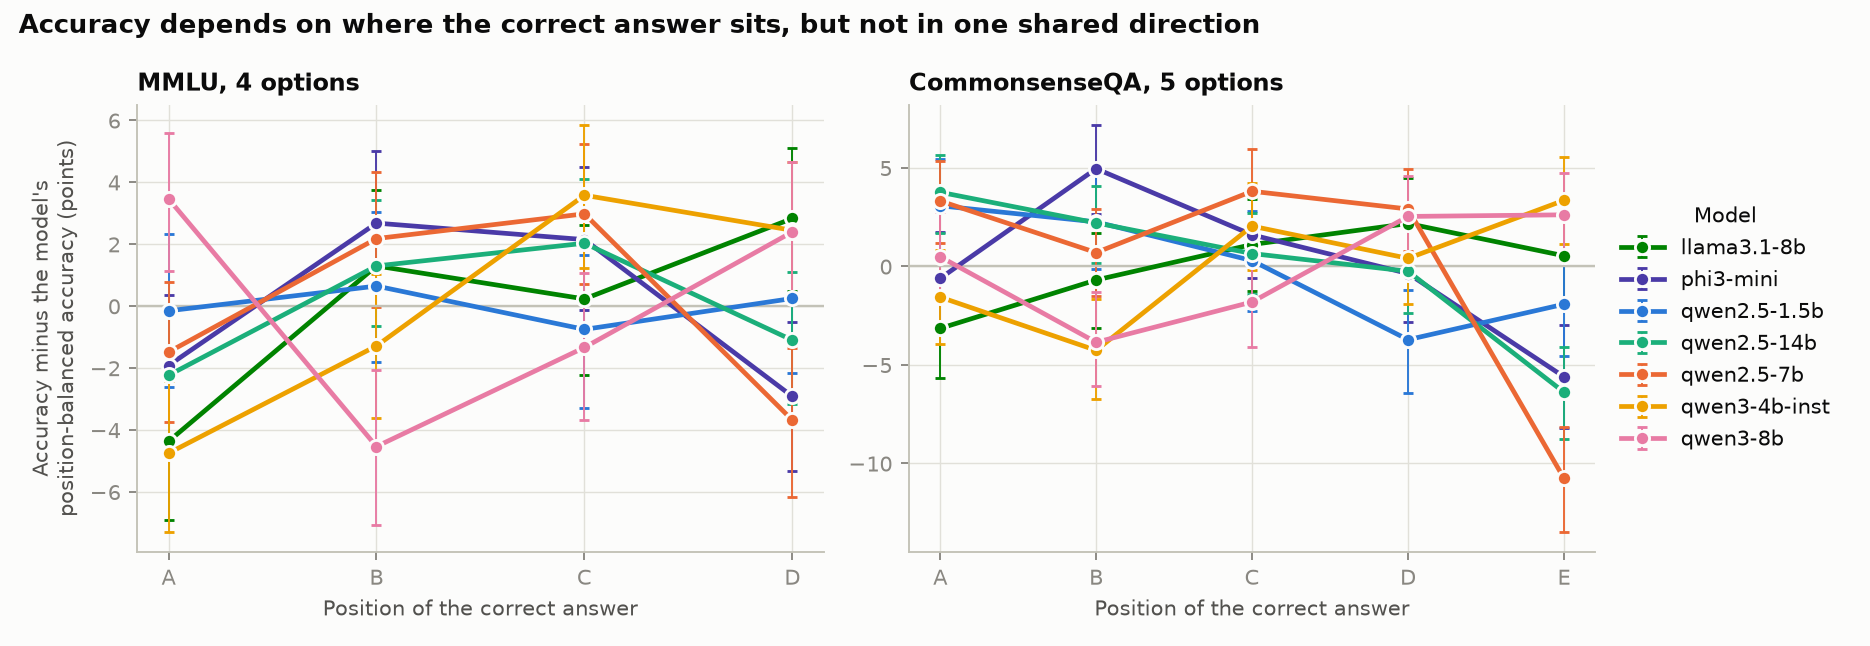
\includegraphics[width=0.95\linewidth]{figures/fig1_accuracy_by_gold_position.png}
    \caption{Accuracy by position of the correct answer, relative to each model's position-balanced accuracy, with 95\% intervals. Left: \mmlu with four options. Right: \csqa with five options. The curves cross: no position is good or bad for all models. On \csqa, the last slot (E) is the worst position for four models and the best for the two Qwen3 models.}
    \label{fig:accpos}
\end{figure}

{\bf Does position change accuracy?}
Yes, for six of seven models.
\Tabref{tab:mmlu_main} shows that the spread on \mmlu is 4.3--8.3 points for these six, against 1.3--1.7 points expected from noise alone, and Cochran's Q rejects position-independence for each of them after Holm correction.
The exception is qwen2.5-1.5b, whose spread of 1.4 is at the noise level.

{\bf Is the effect a preference for A/B?}
No.
Accuracy with the key at A is \emph{below} balanced accuracy, with the interval excluding zero, for five models, and above it for one (qwen3-8b; but see \secref{sec:robust}).
Averaged over A and B, no model gains and two lose (llama3.1-8b $-$1.5, qwen3-4b-inst $-$3.0).
Among the six models with an effect, B or C is the best position for four, D for one, and A for one (\figref{fig:accpos}).

Selection shares tell the same story (\figref{fig:share}).
With a balanced key, llama3.1-8b picks A 21.7\% of the time and D 27.1\%; qwen3-4b-inst picks A 21.5\% and D 27.3\%; qwen3-8b picks A 29.1\%.
Two models (qwen2.5-1.5b, qwen2.5-14b) are not distinguishable from uniform.

{\bf Are these patterns noise?}
No.
In a post hoc split-half check, each model's pattern replicates across two random halves of the questions: the correlation of the four position accuracies is 0.85--0.98 for the six models with a significant effect.
The patterns are stable traits of each model.

\begin{figure}[t]
    \centering
    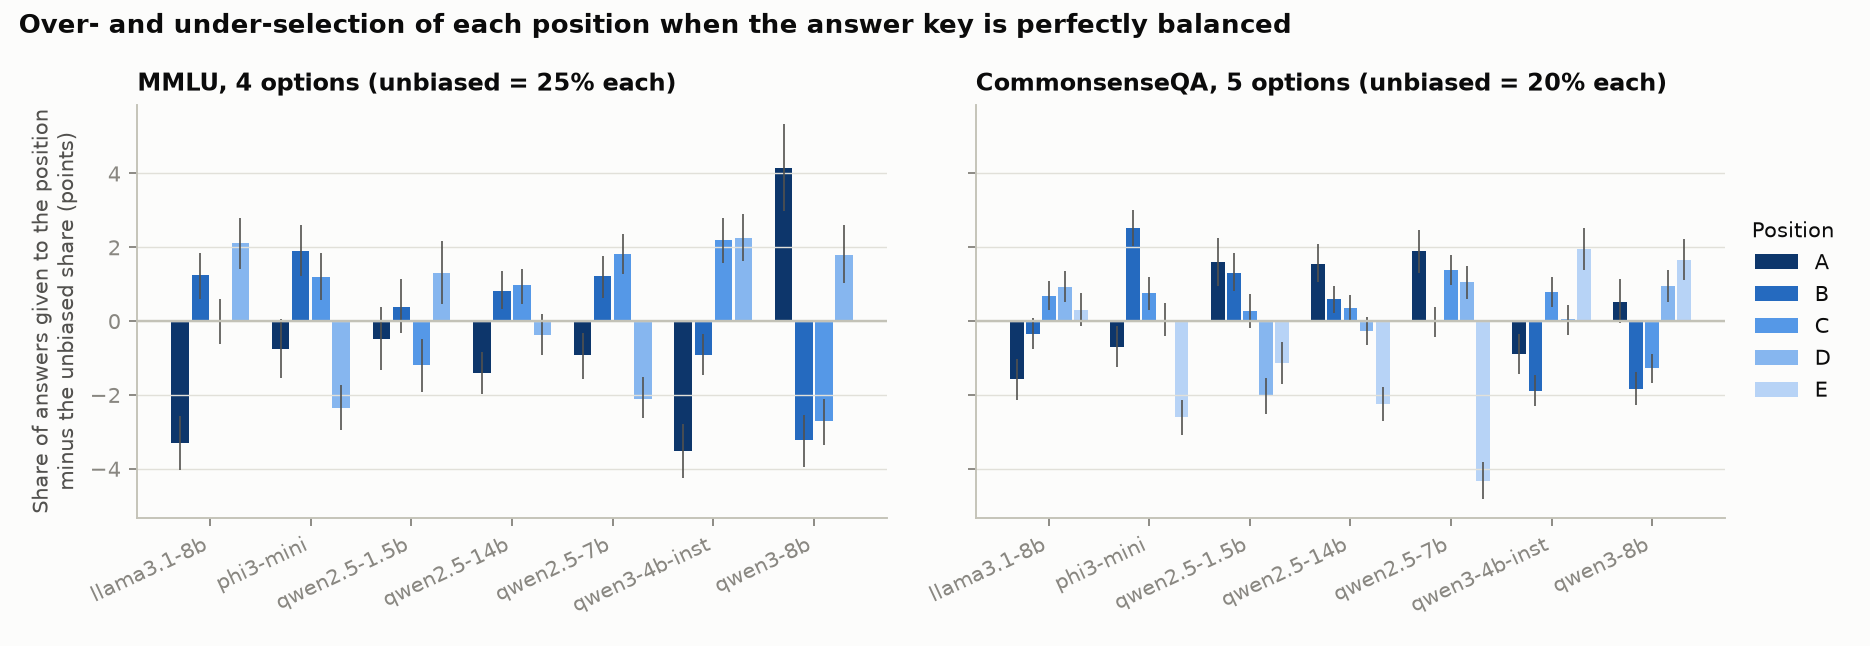
\includegraphics[width=0.95\linewidth]{figures/fig2_selection_share.png}
    \caption{How often each position is chosen, minus the unbiased share, when the answer key is balanced. Bars show 95\% intervals. Models over- and under-select different positions; several under-select A on \mmlu.}
    \label{fig:share}
\end{figure}

\subsection{How much do scores inflate?}
\label{sec:inflation}

\begin{table}[t]
    \centering
    \caption{Three definitions of inflation: accuracy minus position-balanced accuracy, in points, with 95\% bootstrap intervals. Only the best-position definition reaches the low end of the hypothesized 3--8 range, and it is biased upward because the best position is chosen after the fact.}
    \label{tab:inflation}
    \small
    \begin{tabular}{@{}llccc@{}}
        \toprule
        \textbf{Dataset} & \textbf{Model} & \textbf{As published} & \textbf{Key at A or B} & \textbf{Key at best position} \\
        \midrule
        \multirow{8}{*}{\shortstack[l]{\mmlu\\$k{=}4$}}
        & llama3.1-8b   & 0.7 \ci{$-$0.7}{2.0} & $-$1.5 \ci{$-$2.3}{$-$0.8} & 2.8 \ci{1.7}{4.2} \\
        & phi3-mini     & 1.9 \ci{0.7}{3.1}    & 0.4 \ci{$-$0.4}{1.2}       & 2.7 \ci{2.0}{4.0} \\
        & qwen2.5-1.5b  & 2.0 \ci{0.5}{3.5}    & 0.2 \ci{$-$0.6}{1.1}       & 0.6 \ci{0.3}{2.2} \\
        & qwen2.5-7b    & 1.5 \ci{0.4}{2.8}    & 0.3 \ci{$-$0.4}{1.0}       & 3.0 \ci{2.2}{4.1} \\
        & qwen2.5-14b   & 1.2 \ci{0.0}{2.3}    & $-$0.5 \ci{$-$1.1}{0.2}    & 2.0 \ci{1.3}{3.0} \\
        & qwen3-4b-inst & 0.8 \ci{$-$0.3}{2.1} & $-$3.0 \ci{$-$3.8}{$-$2.3} & 3.6 \ci{2.7}{4.7} \\
        & qwen3-8b      & 1.2 \ci{$-$0.1}{2.5} & $-$0.5 \ci{$-$1.3}{0.3}    & 3.5 \ci{2.5}{5.0} \\
        & {\bf Mean of models} & {\bf 1.3} \ci{0.7}{2.0} & {\bf $-$0.7} \ci{$-$1.0}{$-$0.3} & {\bf 2.6} \ci{2.4}{3.2} \\
        \midrule
        \multirow{8}{*}{\shortstack[l]{\csqashort\\$k{=}5$}}
        & llama3.1-8b   & $-$0.2 \ci{$-$1.4}{1.0} & $-$1.9 \ci{$-$2.8}{$-$1.0} & 2.2 \ci{1.3}{3.4} \\
        & phi3-mini     & 1.0 \ci{$-$0.3}{2.2}    & 2.2 \ci{1.3}{3.1}          & 5.0 \ci{3.7}{6.3} \\
        & qwen2.5-1.5b  & 0.3 \ci{$-$1.1}{1.7}    & 2.7 \ci{1.8}{3.6}          & 3.1 \ci{2.0}{4.6} \\
        & qwen2.5-7b    & 0.6 \ci{$-$0.7}{1.9}    & 2.0 \ci{1.2}{2.8}          & 3.8 \ci{3.2}{5.0} \\
        & qwen2.5-14b   & $-$0.2 \ci{$-$1.3}{1.0} & 3.0 \ci{2.2}{3.8}          & 3.8 \ci{2.6}{5.2} \\
        & qwen3-4b-inst & 0.1 \ci{$-$1.2}{1.3}    & $-$2.9 \ci{$-$3.9}{$-$2.0} & 3.4 \ci{2.3}{4.7} \\
        & qwen3-8b      & 0.8 \ci{$-$0.4}{2.2}    & $-$1.7 \ci{$-$2.6}{$-$0.7} & 2.6 \ci{1.9}{3.9} \\
        & {\bf Mean of models} & {\bf 0.3} \ci{$-$0.3}{1.0} & {\bf 0.5} \ci{0.0}{0.9} & {\bf 3.4} \ci{3.1}{4.0} \\
        \bottomrule
    \end{tabular}
\end{table}


\Tabref{tab:inflation} and \figref{fig:inflation} report the three definitions of inflation from \secref{sec:metrics}.

\para{As published.}
\mmlu scores sit 1.3 points \ci{0.7}{2.0} above balanced accuracy on average.
\csqa scores are not distinguishable from balanced (0.3 \ci{$-$0.3}{1.0}).
Both are well short of the hypothesized 3--8 points.

\para{Key at A or B.}
If every key were at A or B, the average model would score slightly \emph{lower} on \mmlu ($-$0.7 \ci{$-$1.0}{$-$0.3}).
On \csqa four models gain 2--3 points and three lose 2--3.

\para{Key at the best position.}
Placing every key at the position a model favors is worth 2.0--3.6 points on \mmlu for the six models with an effect, and 2.2--5.0 on \csqa.
This is the only definition that reaches the low end of the hypothesized range.
It is also biased upward, because we pick the best position after the fact; noise alone gives 0.6--0.9 points.

\begin{figure}[t]
    \centering
    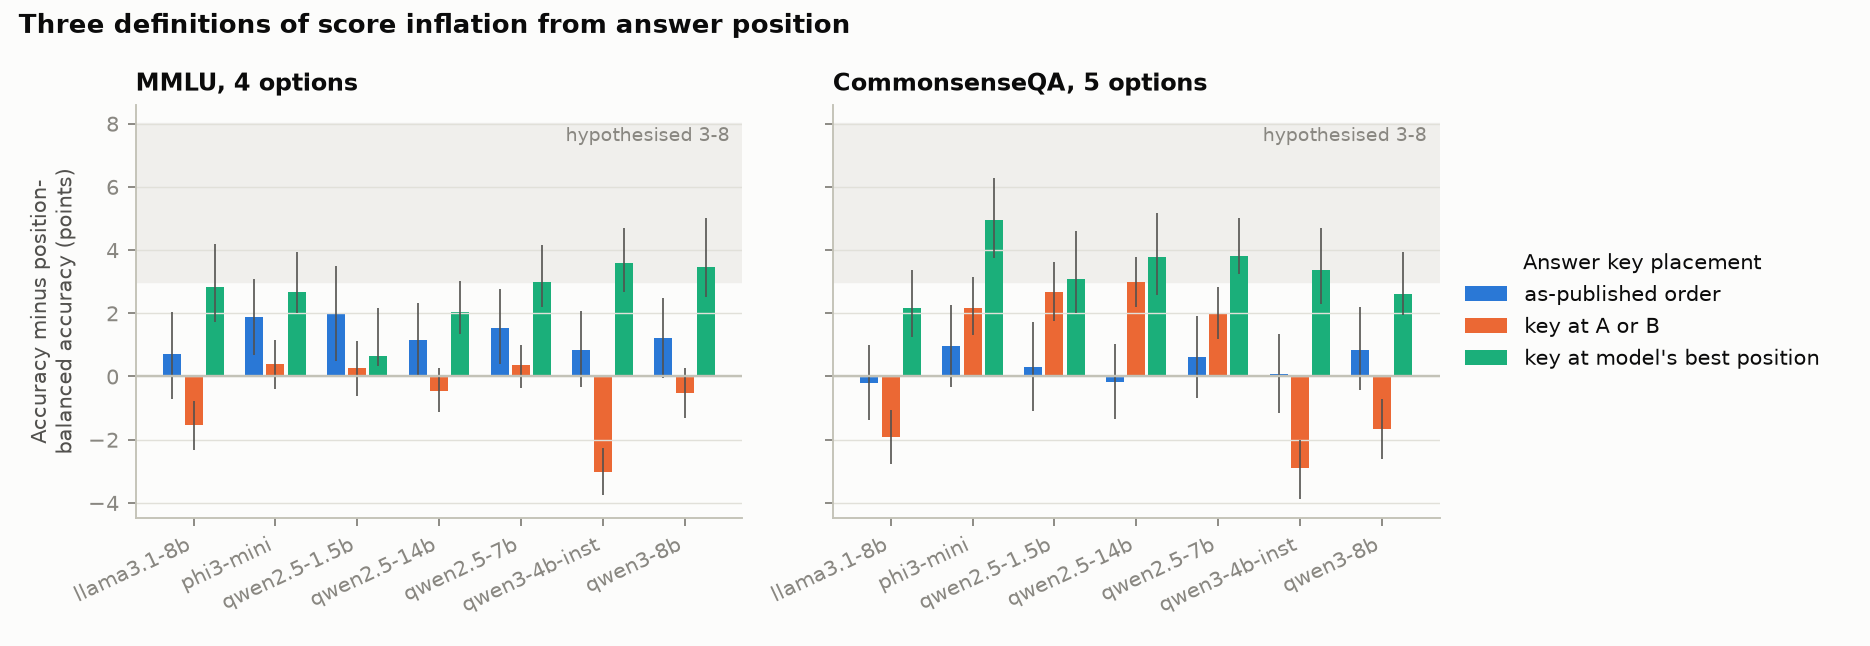
\includegraphics[width=0.95\linewidth]{figures/fig5_inflation_definitions.png}
    \caption{Three definitions of score inflation, per model, with 95\% intervals. The shaded band marks the hypothesized 3--8 points. As-published inflation (blue) stays below the band for every model, and early-key inflation (orange) is negative for several models.}
    \label{fig:inflation}
\end{figure}

{\bf Where do the 1.3 points on \mmlu come from?}
Not from key placement.
In a post hoc decomposition, we weight each model's per-position accuracy by the actual key distribution of our \mmlu sample (A 24.5\%, B 23.8\%, C 25.1\%, D 26.6\%); this predicts a gain of 0.0 \ci{0.0}{0.1}.
The whole 1.3 points therefore reflects that the published arrangement is easier than a rotation with the key in the same slot.
Part of this comes from options that only make sense in their original place, such as ``All of the above'' or ``Both A and B''.
On the 108 questions that a regular expression flags as order-dependent, the as-published advantage is 4.7 \ci{2.4}{7.5} points, against 1.1 \ci{0.5}{1.7} on the other 1{,}392.
The remaining 1.1 points is consistent with models having seen these items in their original order during training, but we cannot separate that explanation from order-dependent options that the regular expression missed.

\subsection{Option count and format}
\label{sec:format}

\begin{table}[t]
    \centering
    \caption{Position effects by format, mean of models with 95\% intervals. Spread is best minus worst position; for two options the best-position gain is half the spread. The two largest spreads (in \textbf{bold}) come from word-answer true/false and from numeric labels, not from the format with the most options. The numeric-label row excludes phi3-mini (\secref{sec:labels}).}
    \label{tab:format}
    \small
    \begin{tabular}{@{}lccccc@{}}
        \toprule
        \textbf{Condition} & \textbf{Models} & \textbf{Balanced acc.} & \textbf{Spread} & \textbf{Best-position gain} & \textbf{Flip \%} \\
        \midrule
        \boolq, True/False words & 7 & 79.5 & {\bf 14.2} \ci{13.5}{15.0} & 7.1 \ci{6.8}{7.5} & 14.6 \\
        \boolq, A/B letters      & 7 & 82.3 & 4.4 \ci{4.1}{4.9}   & 2.2 \ci{2.0}{2.5} & 6.2 \\
        \midrule
        \mmlu $k{=}2$ & 7 & 81.0 & 6.0 \ci{5.2}{6.8} & 3.0 \ci{2.6}{3.4} & 17.9 \\
        \mmlu $k{=}3$ & 7 & 72.2 & 5.7 \ci{5.0}{6.6} & 2.9 \ci{2.4}{3.3} & 24.6 \\
        \mmlu $k{=}4$ & 7 & 67.4 & 5.9 \ci{5.4}{6.9} & 2.6 \ci{2.4}{3.2} & 29.5 \\
        \mmlu $k{=}4$, labels 1--4 & 6 & 64.7 & {\bf 13.6} \ci{12.6}{14.8} & 6.2 \ci{5.7}{6.8} & 37.7 \\
        \midrule
        \csqashort $k{=}2$ & 7 & 91.8 & 2.9 \ci{2.6}{3.7} & 1.5 \ci{1.3}{1.8} & 8.4 \\
        \csqashort $k{=}3$ & 7 & 85.6 & 4.7 \ci{4.0}{5.5} & 2.4 \ci{2.0}{2.8} & 15.4 \\
        \csqashort $k{=}4$ & 7 & 81.4 & 4.6 \ci{4.0}{5.4} & 2.4 \ci{2.1}{2.9} & 21.0 \\
        \csqashort $k{=}5$ & 7 & 77.1 & 8.8 \ci{8.0}{9.9} & 3.4 \ci{3.1}{4.0} & 27.6 \\
        \bottomrule
    \end{tabular}
\end{table}


\begin{figure}[t]
    \centering
    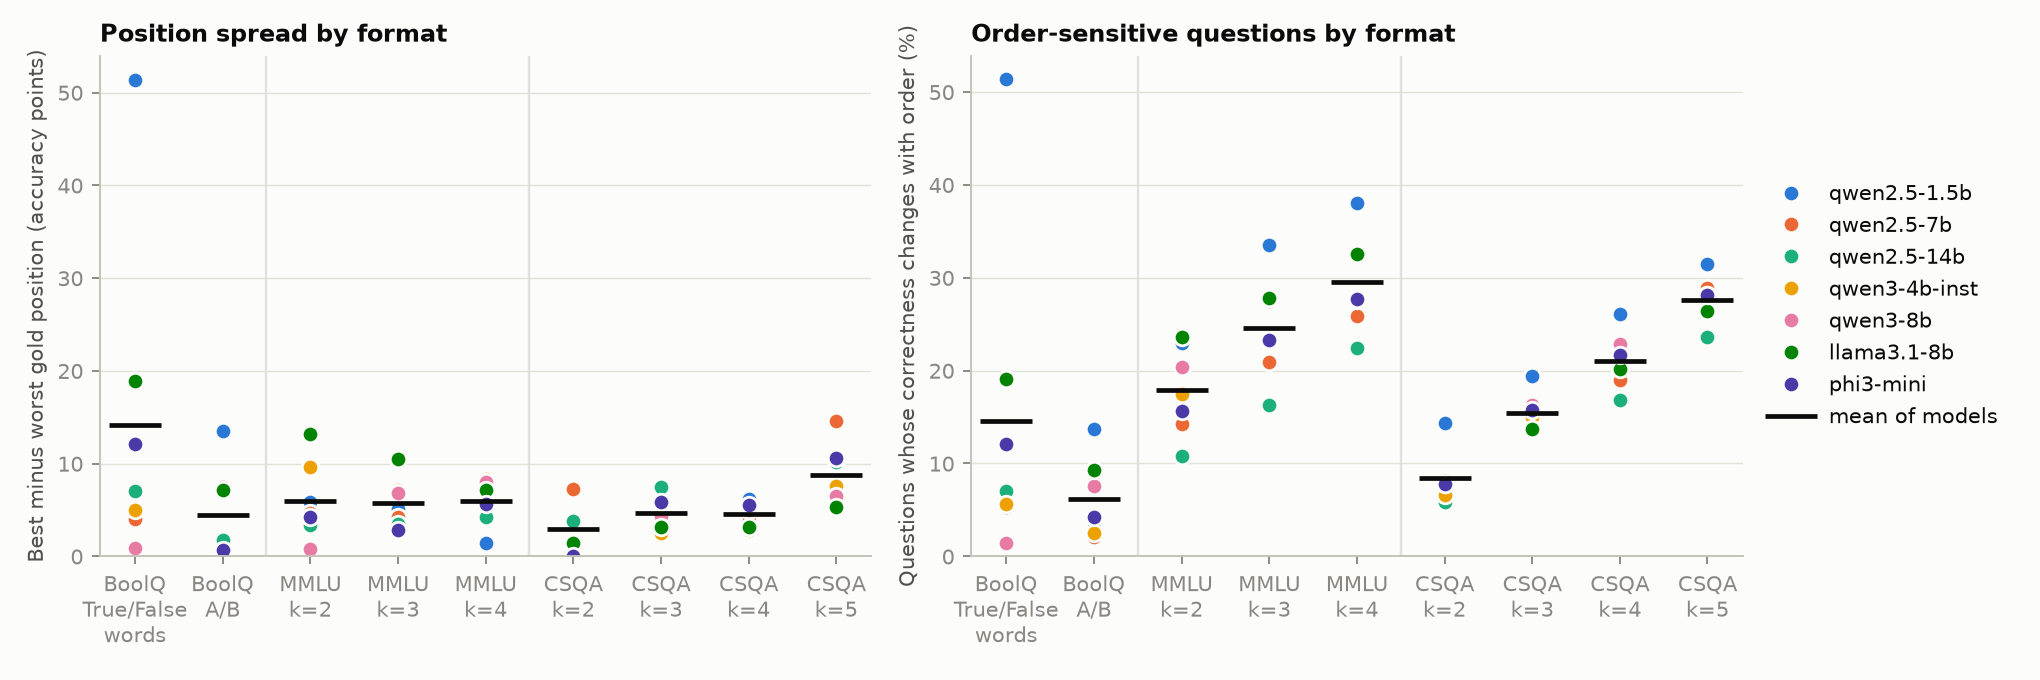
\includegraphics[width=0.95\linewidth]{figures/fig3_format_ladder.png}
    \caption{Position spread (left) and flip rate (right) by format, one dot per model; black bars are means over models. The spread is flat across option counts on \mmlu and jumps at five options on \csqa. The flip rate rises steadily with option count on both datasets. The outlier in the word-answer true/false condition is qwen2.5-1.5b.}
    \label{fig:format}
\end{figure}

\para{True/false is not the safest format.}
With word answers, the mean spread is 14.2 points, the largest in the study (\tabref{tab:format}).
The spread is under 2 points for one of seven models with word answers (qwen3-8b, 0.9) and for four of seven with A/B letters.
It is far above 2 for the rest: with word answers llama3.1-8b is at 18.9, phi3-mini at 12.1, and qwen2.5-1.5b at 51.4.
The last model picks whichever word the instruction mentions first 75.7\% of the time; it scores 90.7\% when the true answer is mentioned first and 39.3\% when it is second.
The direction again varies: four models favor the first-mentioned word and three the second.
With two options there is no averaging over positions, so a preference for one word translates directly into accuracy.

\para{Five options.}
The spread exceeds 10 points for three of seven models (qwen2.5-7b 14.6, phi3-mini 10.6, qwen2.5-14b 10.2) and averages 8.8.
On identical questions, going from four to five options raises the spread by 4.2 \ci{3.3}{4.9} points.
The increase is concentrated in one slot: four models are worse when the key is at E, three of them by 5--11 points (qwen2.5-7b drops 10.8 points below its balanced accuracy there), while both Qwen3 models are \emph{best} at E (\figref{fig:accpos}, right).

\para{Option count on its own does not drive the spread.}
On \mmlu the spread is flat from two to four options ($k{=}4$ minus $k{=}2$: 0.0 \ci{$-$0.9}{1.1}).
What rises steadily with option count on both datasets is the flip rate (\figref{fig:format}, right).
More options mean more questions whose answer changes with order, but those changes mostly cancel rather than favor a position.

\subsection{Difficulty}
\label{sec:difficulty}

\begin{table}[t]
    \centering
    \caption{Position effects by difficulty quintile, mean of models with 95\% intervals. Difficulty for a model is the mean balanced correctness of the other six models. Directed gap is accuracy at the model's overall best position minus its overall worst. The largest directed gap per dataset is in \textbf{bold}. The effect is near zero on easy questions.}
    \label{tab:difficulty}
    \resizebox{\textwidth}{!}{%
    \begin{tabular}{@{}llccccc@{}}
        \toprule
        \textbf{Dataset} & \textbf{Stratum} & \textbf{Balanced acc.} & \textbf{Directed gap} & \textbf{Flip \%} & \textbf{As-published gain} & \textbf{Position-attributable share \%} \\
        \midrule
        \multirow{5}{*}{\mmlu $k{=}4$}
        & Q1 hardest & 19.9 & 7.6 \ci{5.9}{9.5}   & 37.5 & 1.4 \ci{0.2}{2.5}       & 15.6 \ci{14.8}{21.0} \\
        & Q2         & 50.0 & {\bf 11.5} \ci{9.0}{13.8} & 55.6 & 2.7 \ci{1.3}{4.2}       & 9.1 \ci{8.3}{12.2} \\
        & Q3         & 76.3 & 6.3 \ci{4.3}{8.2}   & 34.8 & 2.5 \ci{1.3}{3.6}       & 5.8 \ci{5.1}{7.4} \\
        & Q4         & 93.1 & 3.3 \ci{2.1}{4.6}   & 14.0 & $-$0.2 \ci{$-$0.9}{0.5} & 2.2 \ci{1.8}{3.0} \\
        & Q5 easiest & 97.5 & 0.9 \ci{0.1}{1.7}   & 5.8  & 0.3 \ci{$-$0.1}{0.8}    & 0.8 \ci{0.7}{1.3} \\
        \midrule
        \multirow{5}{*}{\csqashort $k{=}5$}
        & Q1 hardest & 30.0 & {\bf 16.6} \ci{14.2}{18.8} & 49.6 & 0.0 \ci{$-$1.4}{1.7}    & 19.2 \ci{17.1}{23.1} \\
        & Q2         & 71.9 & 14.9 \ci{12.4}{17.3} & 49.4 & 1.3 \ci{$-$0.2}{2.6}    & 8.1 \ci{7.1}{10.0} \\
        & Q3         & 88.9 & 9.1 \ci{7.3}{10.9}   & 25.9 & $-$0.2 \ci{$-$1.4}{0.8} & 4.3 \ci{3.8}{5.5} \\
        & Q4         & 96.7 & 1.5 \ci{0.5}{2.5}    & 8.3  & 0.6 \ci{0.1}{1.2}       & 1.4 \ci{1.2}{2.1} \\
        & Q5 easiest & 98.1 & 1.8 \ci{1.0}{2.6}    & 4.9  & 0.0 \ci{$-$0.4}{0.5}    & 0.9 \ci{0.8}{1.4} \\
        \bottomrule
    \end{tabular}
    }
\end{table}


\begin{figure}[t]
    \centering
    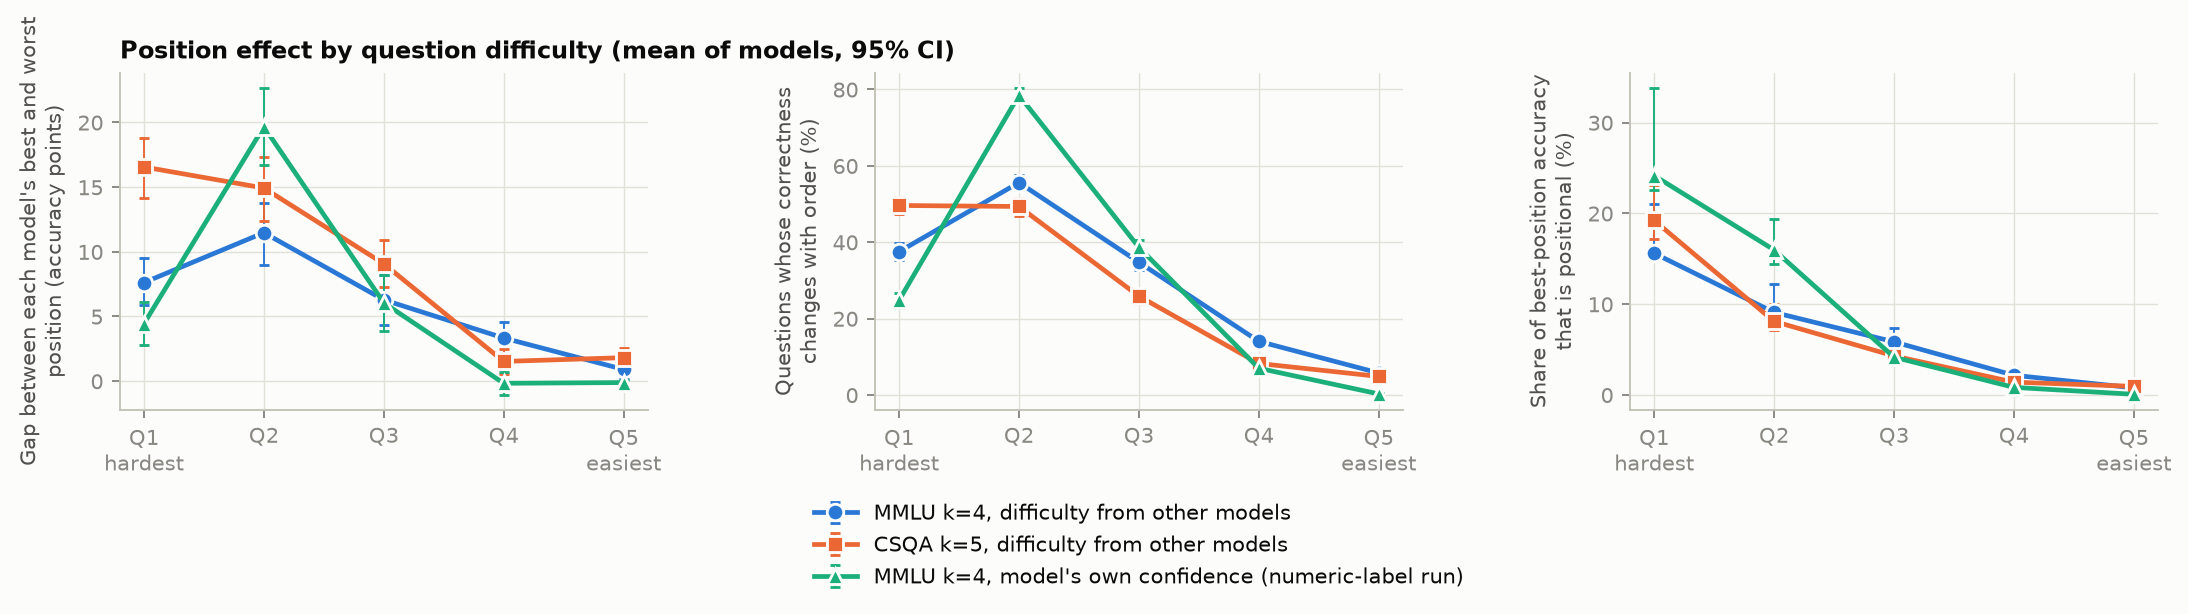
\includegraphics[width=0.95\linewidth]{figures/fig4_difficulty.png}
    \caption{Position effect by difficulty quintile, mean of models with 95\% intervals. Left: directed gap. Middle: flip rate. Right: position-attributable share. With difficulty from the other models, the gap on \mmlu peaks in the second-hardest quintile; with the model's own confidence (green) the peak is sharper.}
    \label{fig:difficulty}
\end{figure}

{\bf Is the effect strongest at medium difficulty?}
Only if ``medium'' means ``near 50\% accuracy''.
\Tabref{tab:difficulty} and \figref{fig:difficulty} show that the position effect is near zero on easy questions and large on hard ones.
When we cut questions into thirds, the middle third is \emph{not} the peak: the hard third exceeds the middle third on directed gap by 3.3 \ci{1.1}{5.7} points on \mmlu and 7.6 \ci{5.2}{9.9} on \csqa.

In quintiles, \mmlu does show a peak, at the second-hardest quintile, where balanced accuracy is 50\%.
The hardest quintile, where accuracy is 20\% and below the 25\% chance rate, has a smaller gap.
On \csqa the two hardest quintiles (30\% and 72\% accuracy) are level.

Each model's own confidence, taken from the separate numeric-label run, gives a sharper version of the same shape on \mmlu.
The gap is 19.7 \ci{16.7}{22.7} points in the quintile where accuracy is 47\%, and 78.5\% of those questions change correctness with order.
It is 4.4 points where accuracy is 8\%, and zero where accuracy is 97\% or more.
The effect therefore tracks uncertainty: it is largest where the model is close to a coin flip between a right and a wrong answer.
On these benchmarks that region is the hard-to-middle part, not the middle.

{\bf What share of accuracy is positional?}
In the hardest quintile, 15.6\% (\mmlu) and 19.2\% (\csqa) of best-position accuracy would disappear under a balanced key; in the hardest third the figures are 13.0\% and 13.4\%.
Single models go higher (qwen2.5-14b on the hardest \csqa quintile: 28\%).
These are best-case figures with the upward bias noted in \secref{sec:inflation}, and the ratios in the hardest strata have small denominators.
Measured on the benchmarks as published, the share is 6.9\% \ci{3.5}{10.1} in the hardest \mmlu third and indistinguishable from zero on \csqa.

\subsection{Label ablation: 1--4 instead of A--D}
\label{sec:labels}

\begin{table}[t]
    \centering
    \caption{Label ablation on \mmlu $k{=}4$: same questions and option order, labels A--D versus 1--4. ``First slot'' is accuracy with the key in the first slot minus balanced accuracy. The larger spread per model is in \textbf{bold}. With numerals, all six models are below balanced accuracy when the key is in the first slot.}
    \label{tab:labels}
    \small
    \begin{tabular}{@{}lcccc@{}}
        \toprule
        & \multicolumn{2}{c}{\textbf{Spread}} & \multicolumn{2}{c}{\textbf{First slot}} \\
        \cmidrule(lr){2-3}\cmidrule(lr){4-5}
        \textbf{Model} & \textbf{A--D} & \textbf{1--4} & \textbf{A--D} & \textbf{1--4} \\
        \midrule
        llama3.1-8b   & 7.2 & {\bf 22.8} & $-$4.4 & $-$14.2 \\
        qwen2.5-1.5b  & 1.4 & {\bf 10.1} & $-$0.1 & $-$3.7 \\
        qwen2.5-7b    & 6.7 & {\bf 7.1}  & $-$1.5 & $-$0.7 \\
        qwen2.5-14b   & 4.3 & {\bf 11.5} & $-$2.2 & $-$6.8 \\
        qwen3-4b-inst & 8.3 & {\bf 15.6} & $-$4.8 & $-$8.9 \\
        qwen3-8b      & 8.0 & {\bf 14.7} & $+$3.5 & $-$7.9 \\
        \bottomrule
    \end{tabular}
\end{table}


We rerun \mmlu $k{=}4$ with the same questions in the same order but with numeric labels.
We exclude phi3-mini from this comparison: it emits a whitespace token before a digit, so the first-token read-out carries no information.
Over the remaining six models, the mean spread rises by 7.7 points \ci{6.4}{8.5}, to 13.6 (\tabref{tab:labels}).
With numerals, all six models are below balanced accuracy when the key is in the first slot; llama3.1-8b scores 48.0\% there against 70.8\% in the second slot.
The size of the order effect thus depends heavily on which symbols label the options.
This fits the token-preference account of \citet{zheng2024selectors} better than a pure position account, although our design does not separate the two further.

\subsection{Does the read-out match what models write?}
\label{sec:readout}

We also answer 400 \mmlu prompts per model by greedy generation.
When the generated text contains a letter, it agrees with the first-token read-out in 97.5--99.8\% of cases across models.
The generated text contains a letter in 95.2--100\% of cases for six models and in 89.0\% for qwen3-8b, which sometimes starts an explanation instead (\tabref{tab:readout} in the appendix).

\subsection{Robustness}
\label{sec:robust}

\para{qwen3-8b is unreliable in direction on \mmlu.}
This model puts less than half of its first-token probability on any letter for at least one rotation of 391 of the 1{,}500 questions.
On the 1{,}109 remaining questions its spread is similar (7.2 versus 8.0), but the sign at position A flips, from $+$3.5 to $-$3.3.
Its apparent preference for A in \secref{sec:fouropt} is thus produced by questions where it was not going to answer with a letter.
For the other six models, the spread, the as-published gain, and the position-A effect each change by under 1 point under the same filter.

\para{Batch-composition noise.}
Rerunning qwen2.5-1.5b on 3{,}000 prompts with different batching reproduces 99.1\% of predictions; label log-probabilities move by 0.11 on average.
This comes from bfloat16 arithmetic with padded batches.
It adds up to about a point to flip rates and is unrelated to position.

\para{Multiple comparisons.}
Cochran's Q is significant after Holm correction in 57 of 70 model-by-condition cells, including 6 of 7 on \mmlu $k{=}4$ and 7 of 7 on \csqa $k{=}5$.

\section{Discussion}
\label{sec:discussion}

\begin{table}[t]
    \centering
    \caption{Verdicts on the five hypotheses fixed before the experiments.}
    \label{tab:verdicts}
    \small
    \begin{tabular}{@{}lp{0.23\textwidth}p{0.17\textwidth}p{0.47\textwidth}@{}}
        \toprule
        & \textbf{Claim} & \textbf{Verdict} & \textbf{Evidence} \\
        \midrule
        H1 & Consistent bias toward A/B & {\bf Not supported} & Position effects are real in 6/7 models but point in different directions; on \mmlu 5/7 are below their average at A. \\
        H2 & 3--8 points inflation on 4-option items & {\bf Not supported} & As published $+$1.3 \ci{0.7}{2.0}, none of it from key placement; A/B key $-$0.7; best case 2.0--3.6. \\
        H3 & Strongest at medium difficulty & {\bf Partly supported} & Strongest where the model is near 50\% accuracy; this is the hard-to-middle range, and the middle third is weaker than the hard third. \\
        H4a & True/false $<$2 points & {\bf Not supported} & Mean spread 14.2 (words) and 4.4 (letters); under 2 for 1/7 and 4/7 models. \\
        H4b & 5-option $>$10 points, the largest & {\bf Partly supported} & Spread $>$10 for 3/7 models, mean 8.8; larger than 4-option on the same questions, but smaller than true/false words and numeric labels. \\
        H5 & Up to 15\% of accuracy near the boundary & {\bf Best case only} & 13--19\% in the hardest strata if every key sat at the model's favored position; 7\% or less as published. \\
        \bottomrule
    \end{tabular}
\end{table}


\Tabref{tab:verdicts} summarizes the verdicts on the five hypotheses.

{\bf Why is ``inflation'' mostly the wrong word?}
A position preference only raises a score when the benchmark's keys are concentrated where the model likes to answer.
\mmlu and \csqa have close-to-uniform keys, so the preferences largely cancel.
What the preferences do produce is \emph{instability}: about 30\% of \mmlu questions and 28\% of \csqa questions are answered correctly under some option orders and incorrectly under others.
This matters for per-question analyses and for small benchmarks, and it would matter for aggregate scores on any benchmark with a skewed key.

\para{Surprises.}
First, the simplest format produced the largest effect: word-answer true/false gives a 14.2-point spread on average.
Second, position A is a disadvantage, not an advantage, for five of these seven models on \mmlu.
Third, the published \mmlu order is 1.3 points easier than its rotations for reasons unrelated to where the key is.
This is a caution for any shuffle-based debiasing: rotating options also damages order-dependent items.

\para{Relation to prior work.}
The model-specific direction, the dependence on label tokens, and the growth of the effect with uncertainty are in line with the findings of \citet{zheng2024selectors} for earlier models.
This comparison is qualitative: we did not rerun prior methods, and we did not conduct a systematic literature review for this study.

\para{Implications for evaluation practice.}
\begin{itemize}[leftmargin=*,itemsep=0pt,topsep=0pt]
    \item Report position-balanced accuracy ($k$ rotations) when comparing models whose scores differ by a few points.
    \item Check the answer-key distribution of any new benchmark; a skewed key is where a 2--5 point distortion would actually appear.
    \item Do not assume two-option or true/false items are immune; test both orders.
    \item Treat per-question correctness as order-dependent for roughly a quarter to a third of items.
\end{itemize}

\subsection{Limitations}
\label{sec:limitations}

\para{Model coverage.}
We study seven open-weight models, none above 14B parameters, five from one vendor.
We planned to run hosted frontier models and could not.
Larger models may be less order-sensitive: within Qwen2.5 the true/false word effect shrinks from 51 points at 1.5B to 4--7 points at 7B and 14B.
Our numbers should not be read as applying to frontier models.

\para{Rotations, not full shuffles.}
Cyclic rotation balances key position with $k$ prompts per question but covers $k$ of $k!$ orders, and it moves order-dependent options out of place.
About 7\% of our \mmlu sample is affected; we did not validate by hand the regular expression that flags these questions.

\para{Position versus label.}
Position and label are tied in every condition except the single A--D versus 1--4 comparison.
We show that the effect is label-dependent but do not apportion it between the two.

\para{First-token read-out.}
Agreement with generated text is 97.5--99.8\% where the model writes a letter, but qwen3-8b and, with numerals, phi3-mini do not reliably start with a label.

\para{One prompt template, zero-shot.}
We did not test few-shot prompts, other instructions, or chain-of-thought answers, all of which may change selection behavior.

\para{True/false is one dataset with one unusual phrasing.}
Our \boolq items are passage-based and use the statement ``The answer to the question \ldots\ is yes.''
The large word-order effect may not carry over to plain factual true/false statements.

\para{Contamination.}
\mmlu, \csqa, and \boolq are very likely in these models' training data.
The 1.1-point residual advantage of the published \mmlu order may reflect this.

\para{Best-position figures are biased upward.}
We choose the best position from the same data.
The noise-only reference (0.6--0.9 points on the full sets) is larger in the smaller difficulty strata.

\para{Difficulty from other models.}
Our difficulty measure is a property of this particular set of seven models and is correlated across the five Qwen models.

\para{Post hoc analyses.}
The decomposition of the as-published gain, the order-dependent split, the split-half replication, the permutation null, and the low-label-mass filter were added after we saw the results.

\section{Conclusion}
\label{sec:conclusion}

We test whether instruct LLMs favor early answer positions and whether this inflates multiple-choice scores, using a within-question rotation design on seven open-weight models and three benchmarks.
Answer order changes what these models answer, but not in the way the hypothesis states.
There is no shared preference for early positions: each model has its own stable pattern, and most do worse than their own average at A on \mmlu.
Because benchmark keys are close to uniform, the net effect on published scores is about one point or less.
The effect is concentrated on questions where the model is close to 50/50, is larger with five options than four because of the last slot, is largest for word-answer true/false in small models, and depends strongly on the label symbols.

The key takeaway is that, for these models, answer position makes multiple-choice scores unstable at the question level rather than inflated in aggregate.

Future work should, in order of value: rerun the same items on hosted frontier models with a generated-text read-out; separate label from position with a crossed design in which labels are permuted independently of slots; use full random shuffles on self-contained questions only, to remove the order-dependent-option confound; test whether the residual advantage of the published \mmlu order appears on a benchmark released after the models' training cut-offs; and repeat the true/false experiment with plain factual statements and several phrasings.


\bibliography{references}

\appendix
\section{Experimental details}
\label{app:setup}

\para{Models and hardware.}
\Tabref{tab:models} lists the model repositories.
We run all models locally with HuggingFace \texttt{transformers} in bfloat16, each on one RTX A6000 (48\,GB).
We left Gemma models out because their tokenizer files were not available to us.
GPU time for the scored runs was about 1.9 hours in total (4 to 29 minutes per model on a shared machine, so timings are not comparable across models).
The analysis takes about 10 minutes on CPU and reproduces every table exactly from a fixed seed.

\begin{table}[h]
    \centering
    \caption{Models. We use the unsloth mirror of Meta's Llama-3.1-8B-Instruct weights.}
    \label{tab:models}
    \small
    \begin{tabular}{@{}lll@{}}
        \toprule
        \textbf{Tag} & \textbf{HuggingFace repository} & \textbf{Family} \\
        \midrule
        qwen2.5-1.5b  & \texttt{Qwen/Qwen2.5-1.5B-Instruct} & Qwen \\
        qwen2.5-7b    & \texttt{Qwen/Qwen2.5-7B-Instruct} & Qwen \\
        qwen2.5-14b   & \texttt{Qwen/Qwen2.5-14B-Instruct} & Qwen \\
        qwen3-4b-inst & \texttt{Qwen/Qwen3-4B-Instruct-2507} & Qwen \\
        qwen3-8b      & \texttt{Qwen/Qwen3-8B} (thinking disabled) & Qwen \\
        llama3.1-8b   & \texttt{unsloth/Meta-Llama-3.1-8B-Instruct} & Llama \\
        phi3-mini     & \texttt{microsoft/Phi-3-mini-4k-instruct} & Phi \\
        \bottomrule
    \end{tabular}
\end{table}

\section{Prompt templates}
\label{app:prompts}

Lettered multiple-choice items (shown here with four options):

\begin{lstlisting}
{question}

A. {option}
B. {option}
C. {option}
D. {option}

Answer with the letter of the correct option only.
\end{lstlisting}

\boolq with word answers. The reversed order mentions ``False or True'' instead. The A/B-letter condition replaces the last line with the two lettered options and the letter instruction.

\begin{lstlisting}
Passage: {passage}

Statement: The answer to the question "{question}?" is yes.

Is the statement True or False? Answer with one word only: True or False.
\end{lstlisting}

\section{Read-out validation}
\label{app:readout}

\begin{table}[h]
    \centering
    \caption{Greedy generation on 400 \mmlu prompts per model, compared with the first-token read-out. Agreement is computed on the prompts where the generated text contains a letter.}
    \label{tab:readout}
    \small
    \begin{tabular}{@{}lcc@{}}
        \toprule
        \textbf{Model} & \textbf{Generated text contains a letter \%} & \textbf{Agreement with read-out \%} \\
        \midrule
        llama3.1-8b   & 99.8  & 98.2 \\
        phi3-mini     & 95.2  & 97.6 \\
        qwen2.5-1.5b  & 97.5  & 99.5 \\
        qwen2.5-7b    & 100.0 & 98.2 \\
        qwen2.5-14b   & 99.2  & 99.8 \\
        qwen3-4b-inst & 95.5  & 99.7 \\
        qwen3-8b      & 89.0  & 97.5 \\
        \bottomrule
    \end{tabular}
\end{table}


\end{document}
